\documentclass[utf8]{gradu3}
% Jos työ on kandidaatintutkielma eikä pro gradu, käytä ylläolevan asemesta
%\documentclass[utf8,bachelor]{gradu3}
% Jos kirjoitat englanniksi, käytä ylläolevan asemesta
%\documentclass[utf8,english]{gradu3}
% tai
%\documentclass[utf8,bachelor,english]{gradu3}

\usepackage{graphicx} % kuvien mukaan ottamista varten

\usepackage{amsmath} % hyödyllinen jos tekstisi sisältää matikkaa,
                     % ei pakollinen
\usepackage{enumitem} % Paremmat listat
\usepackage{booktabs} % hyvä kauniiden taulukoiden tekemiseen
\usepackage{textgreek} % tarvitaan kreikkalaisille kirjaimille
\usepackage{comment} % paketti suurille kommenttilohkoille
\usepackage{float} % Pitäisi auttaa taulukoiden asettelussa
\usepackage{longtable} % Isommille taulukoille
\usepackage{makecell}

% HUOM! Tämän tulee olla viimeinen \usepackage koko dokumentissa!
\usepackage[bookmarksopen,bookmarksnumbered,linktocpage]{hyperref}

\addbibresource{malliopas.bib} % Lähdetietokannan tiedostonimi

% Estää tekstin pommpimisen marginaalien yli, mutta voi aiheuttaa muita ongelmia.
\sloppy

\begin{document}

\title{Laadullinen simulointi tieteellisenä menetelmänä: Systemaattinen kirjallisuuskartoitus}
\translatedtitle{Qualitative simulations as scientific research method: Systematic literature mapping}
\studyline{Tietotekniikka}
\avainsanat{%
  Laadullinen tutkimus,
  Simulaatio,
  Laadullinen simulaatio,
  Systemaattinen kirjallisuuskartoitus
  }
\keywords{Qualitative research, Simulation, Qualitative simulation, Systematic mapping study}
\tiivistelma{%
Määrällinen simulaatio tarvitsee paljon numeerista taustatietoa järjestelmän toiminnasta,
verrattuna laadulliseen simulaatioon, 
joka mahdollistaa simuloinnin vaikka järjestelmän toiminnan tarkasta tiedossa on puutteita.
Tässä tutkimuksessa toteutettiin kirjallisuuskartoitus
laadullisten simulaatioiden käytöstä tieteellisenä menetelmänä 
ja miten laadullisia simulaatioita pyrittiin käyttämään 
kerätyn aineiston tutkimuksissa. Kirjallisuuskartoituksen tuloksena tuotettiin 
laaja kuvaus laadullisten simulaatioiden käytöstä eri tieteenaloilla.
Kartoituksessa tunnistettiin yhteensa 17 eri tieteenalaa ja 
9 erillaista laadullisilla simulaatioilla haettua tavoitetta. 
Lisäksi kartoituksen aineistosta löydettiin lukuisia eri työkaluja
laadullisten simulaatioiden luomiseen. Keskeisimpinä havaintona todettiin, että laadullisilla
simulaatioilla pyritään usein vähentämään kohdejärjestelmän tietoisuuden aukkoja. Eniten simulaatioita on käytetty kemian tieteiden, tekniikan ja materiaalien tieteiden 
aloilla. Yleisimpiä työkaluja simulaatioiden toteutuksessa
ovat QSIM algoritmi ja Matlab-sovellus. 
}
\abstract{%
Quantitative simulation requires a lot of numerical information about the system's operations,
while qualitative simulation allows simulation even if there is a lack of precise information about the system's operations. 
This study conducted a systematic literature mapping study
on the use of qualitative simulations as
a scientific method and how qualitative simulations were used in studies of collected data. 
The systematic literature mapping study resulted in 
a comprehensive description of the use of
qualitative simulations in different scientific disciplines. 
The literature mapping study identified a total of 17 different disciplines and different objectives pursued by qualitative simulations. 
In addition, the mapping data identified a wide range of tools
for creating qualitative simulations. 
The main findings were that qualitative simulations often aim to reduce gaps in the knowledge of the target system.
Simulations have been most widely used in the fields of chemical sciences, engineering and material sciences. 
The most common tools used to implement simulations
are the QSIM algorithm and the Matlab application.
}

\author{Jaakko Palm}
\contactinformation{\texttt{jaakko.j.palm@student.jyu.fi}}
% jos useita tekijöitä, anna useampi \author-komento
\supervisor{Timo Tiihonen}
% jos useita ohjaajia, anna useampi \supervisor-komento

\maketitle

\mainmatter

\chapter{Johdanto} \label{johdanto}
Tutkimukset jaetaan yleisesti empiirisiin ja teoreettisiin tutkimustyyppeihin.
Empiirisessä tutkimuksessa tehdään ja kerätään havaintoja, sekä analysoidaan 
ja mitataan tutkimuksen kohteena olevaa tapahtumaa tai järjestelmää. 
Tutkimusmenetelmät empiirisille tutkimuksille voivat olla 
tyypiltään \textit{laadullisia (eng. qualitative)} 
tai \textit{määrällisiä (eng. quantitative)}. 
Vertauksena teoreettisessa tutkimuksessa pyritään hahmottamaan 
malleja ja rakenteita aiemman tutkimuskirjallisuuden pohjalta. 
Tämän tutkimuksen kannalta oleellisin ero määrällisen ja laadullisen tutkimuksen 
välillä on tutkimuksesta saatu tulos.
Määrällisessä tutkimuksessa tulos pyritään esittämään lukuina ja niiden virherajoina,
eli puhutaan \textit{määrällisesta datasta (eng. quantitative data)}. 
Laadullisessa tuloksesta saatua tai koostettua dataa ei taas kyetä esittämään 
lukuina tai niiden virherajoina. Näissä tapauksissa puhutaan 
\textit{laadullisesta datasta (eng. qualitative data)}.

On olemass myös kolmas tutkimustyyppi nimeltään laskennallinen tiede, 
mikä koostuu teoreettisten mallien pohjalta rakennetuista numeerisista kokeista. 
Simulointi on menetelmä, jota voidaan käyttää tutkimuksissa.
Simulointi menetelmänä omaa empiirisen ja teoriittisen tutkimuksien piirteitä.
Empiirisen tutkimuksen suhteen simuloinnilla voidaan tutkia ja kerätä havaintoja
kohteena olevasta järjestelmästä, mutta simulointia ei 
kuintenkaan voi kutsua aidosti empiiriseksi,
koska simulointi tarvitsee vahvan teoreettisen pohjan taustalleen.
Laskennallinen tiede perustuu simulointiin, 
koska simulointi vahvasti pohjautuu teoreettisten mallien numeeriseen käsittelyyn.
Simulointia varten yleensä luodaan on ohjelma, 
jolla pyritään jäljittelemään reaalimaailman järjestelmän käyttäytymistä.
Tätä ohjelmaa kutsutaan simulaatioksi.
On olemassa myös muunlaisia simulointitapoja kuin tietokoneella ajettavat ohjelmat, mutta 
tässä tutkimuksessä keskitytään tietokoneella ajattaviin simulaatio-ohjelmiin.

Simulaatiot perustuvat luotuihin malleihin, 
jotka pyrkivät kuvaamaan halutun kohteen käyttäytymistä. 
Mallin luomista kutsutaan mallintamiseksi, joka on erittäin tärkeä prosessi simulointia,
sillä se määrittää mitä ja miten tutkittavaa järjestelmää simuloidaan. 
On useita eri tapauksia joissa järjestelmän muuttamiseksi malliksi 
on tarve toteuttaa niin sanottu laadullinen malli, koska kohteesta tiedetään vain laadullisia riipuvuuksia, eikä määrällisten riippuvuuksien määrittely ole mahdollista.
Esimerkiksi tapauksissa joissa tiedetään kahdella 
kohteen ominaisuudella olevan riippuvuus, 
mutta riippuvuuden tarkkoja numeerisia arvoja ei tiedetä.

Laadulliset mallit ovat hyödyllisiä tapauksissa, joissa halutaan luoda uutta teoriaa ja teorian ennusteita simuloimalla. Vertaamalla laadullisen simulaation tuloksia havaintoihin 
voidaan mahdollisesti selittää mikä mekanismi tai tapahtuma tuottaa havaitun käyttäytymisen jossakin tapauksessa.
Laadullisia malleja voidaan myös käyttää tapauksissa, joissa ei ole yhteistä aukotonta teoriaa ja halutaan tarkastella monimutkaisten ilmiöiden yhteisvaikutuksen seuraamuksia simulaatiolla.

Simulaatioilla kyetään keräämään dataa ja havaintoja tutkittavasta aiheesta suhteellisen helposti ja halvalla, mikä tekee siitä oleellisen tutkimusmenetelmän tieteellisiin tutkimuksiin. Yksinkertaisimmillaan simulaatio on ohjelma, jonka avulla voidaan jäljitellä järjestelmän toimintaa. Ohjelmalle syötetään tapahtuman muuttujat ja ohjelma antaa lopputuloksen siitä, mitä simulaation mallin mukaan tulisi tapahtumaan. 

Simulaatioiden avulla tutkijat voivat suorittaa kokeita, jotka voivat olla epäkäytännöllisiä tai mahdottomia todellisessa maailmassa, säilyttäen samalla laajan tilastollisen analyysin. Koska määrällisessä tutkimuksessa pyritään selittämään ilmiöitä perustuen dataan ja datan väliseen suhteeseen, niin  simulointi on erittäin oleellinen menetelmä määrällisille tutkimuksille. 
Simulaatioiden käyttö laadullisissa tutkimuksissa on monimutkaisempi asia, 
jonka mahdollisuus taas riippuu laadullisen tutkimuksen tyypistä ja kohteesta. 
Simulaatioiden käyttö laadullisissa tutkimuksissa on kuitenkin laaja alue, 
esimerkiksi \textcite{eldabi2002quantitative} ehdottivat tutkimuksessaan miten simulaatioilla voidaan välttää laadullisten menetelmien tyypillisiä ongelmia, kuten työlästä datan keruuta. 

Termi \textit{laadullinen simulaatio (eng. qualitative simulation)},
viittaa simulaatioihin, 
jotka eivät tarvitse tarkkoja numeerisia parametreja toimiakseen. 
Toisin sanoen voidaan simuloida käyttäen laadullista dataa, mikä tekee 
laadullisista simulaatioista oleellisen menetelmän laadullisille tutkimuksille. 
Samoin kuin määrälliset simulaatiot, laadulliset simulaatiot myös perustuvat malleihin.

Tämän tutkimuksen tavoitteena on selvittää miksi laadullisia simulaatioita 
ollaan käytetty tieteellisissä tutkimuksissa. Tämän tiedon saamiseksi on
toteutettu systemaattinen kirjallisuuskartoitus 
laadullisten simulaatioiden käytöstä ja kerätyn aineiston perusteella vastataan 
seuraavaan kysymykseen:
\begin{itemize}
    \item Millaisia tuloksia laadullisilla simulaatioilla pyritään hakemaan?
\end{itemize}

Tutkimuksessa halutaan myös selvittää missä ja miten laadullisia simulaatioita
ollaan käytetty. Tätä varten pyritään vastaamaan myös seuraaviin kysymyksiin:
\begin{itemize}
    \item Minkä alan tutkimuksissa on eniten käytetty laadullisia simulaatioita?
    \item Mitä eri työkaluja löytyy laadullisten simulaatioiden luomiseen?
\end{itemize}

Luvussa 2 kerrotaan simulaatioista ja laadullisista simulaatioista yleisesti. Luvussa 3 käydään läpi tutkimuksen asetelma ja käytetyt menetelmät. Luvussa 4 esitellään kirjallisuuskartoituksen tulokset. Luvussa 5 pohditaan tulosten merkitystä ja luvussa 6 on tutkimuksen yhteenveto.

\chapter{Mallintaminen ja simulaatiot}
Tässä luvussa käydään läpi tutkimuksen kartoitukselle oleellisten asioiden taustaa. 
Simulaatiot perustuvat aina malleihin. Mallien suunnittelemista ja luomista 
kutsutaan mallintamiseksi. Alalussa \ref{mallintaminen} kerrotaan tarkemmin 
mallintamisesta ja sen merkityksestä simuloinnin näkökulmasta. 
Tämän jälkeen katsestetaan itse simulointia ja simulaatioita.
Simulaatio on ollut käsitteenä jo pitkän aikaa, joten alaluvussa
\ref{simulaatio} käydään lyhyesti läpi tutkimukselle oleellinen simulaation historia, 
kehitys ja mitä erityyppisiä simulaatioita on olemassa. 
Laadullinen simulaatio on itsessään liian laaja alue käydä samassa alaluvussa, joten
luvussa \ref{laadullinen simulaatio} tutustutaan tarkemmin 
mikä on laadullinen simulaatio, mitkä ovat sen käyttötarkoituksia 
ja mitä hyötyjä laadullisen simulaation käytössä voi olla. 
Lisäksi laadullisten simulaatioiden luomiseen tarkoitetuista työkaluista annetaan 
muutama yleinen esimerkki.

\section{Mallintaminen} \label{mallintaminen}
Mallintaminen on prosessi jolla pyritään tuottamaan malli, joka jäljittelee 
ja edustaa kiinostuksena olevan järjestelmän toimintaa \parencite{maria1997introduction}. 
Mallintamisen kontekstissa järjestelmä viittaa reaalimaailman osioon, 
joka on tarkasteltavissa erillisenä muusta ympäristöstä.
Mallin tarkoitus on auttaa ennustamaan järjestelmän toimintaa ja muutoksia.
Esimerkkinä malli voi toimia \textit{input-output} ajattelun kautta, 
eli mallille annetaan \textit{syötearvoja (eng. input)} ja malli antaa näiden perusteella
\textit{tulosarvoja (eng. output)} mitä mallin mukaan tulee tapahtumaan.

\textcite{maria1997introduction} mukaan parhaimmat mallit pitävät 
sisällään kiinnostuksena olevan järjestelmän 
ominaisuuksista ja toiminnallisuuksista vain tarpeelliset, 
jotta mallien ymmärtäminen ja testaaminen ei olisi liian monimutkaista.

\textcite{maria1997introduction} mukaan mallintaminen on keskeinen osa simulaatiotutkimuksessa.
Simulaatiota varten luotua mallia kutsutaan simulaatiomalliksi.
Simulaatiomalleja on useita eri tyyppejä, kuten deterministinen malli, 
jossa samoilla syötteillä saadaan aina sama lopputulos, 
sekä stokastinen malli, jossa ainakin yksi syöte- tai tulosmuuttuja on satunnainen. 
Mallit voivat olla myös staattisia, jolloin ajankulua ei oteta huomioon, 
tai dynaamisia, jolloin ajankulu vaikuttaa muuttujiin \parencite{maria1997introduction}. 
Simulaatiot usein perustuvat simulaatiomalleihin. 
Hyvä simulaatiomalli sisältää parametreja,
jotka mahdollistavat mallin uudelleenkäyttämisen \parencite{introduction2005simulation}. 

\textcite{maria1997introduction} mukaan simulaatiomallit koostuvat usein seuraavista komponenteista: järjestelmäkokonaisuudet, syöttemuuttujat, suorituskyvyn mittaajat,
ja osien toiminnalliset suhteet. Mallintamisprosessi tiivistetysti etenee askeleittain, alkaen ongelman tunnistamisella ja muotoilulla, 
jonka perusteella toteutetaan datan keruu. Malli muotoillaan ja kehitetään, 
aikaisempiin askeleihin ja kerättyyn dataan perustuen. Mallin toiminta myös validoitaan tässä vaiheessa. 
Lopuksi mallin toiminta ja logiikka dokumentoidaan myöhempää käyttöä varten.

\section{Simulaatio} \label{simulaatio}
Simulaatio viittaa reaalimaailman prosessin tai 
järjestelmän jäljittelyyn \parencite{banks1999introduction}. 
Käsitteenä simulaatio on ollut jo useampaa sataa vuotta 
\parencite{HistoryOfSimulation}, 
mutta tässä tutkimuksessa keskitytään tietokonesimulointiin, 
joka on saanut alkunsa 1950-luvulla. 
%
\parencites%
    {HistoryOfSimulation}%
    {historyOfSimulation1996}
\relax

Simulaatiotyypit voidaan jakaa aikariippuvaisiin ja ei-aikariipuvaisiin malleihin.
Yksinkertainen esimerkki ei-aikariippuvaisesta simulaatiosta on esimerkiksi staattinen 
syöte-tulos
\textit{Monte Carlo simulaatio}, joka on yksi varhaisimmista simulaatiomenetelmistä
\parencites%
    {historyOfSimulation1996}%
    {historyOfMonte}
\relax
%
. 
Monte Carlo sai nimensä vuonna 1947 \parencite{historyOfMonte}
ja se perustuu tilastotieteeseen ja todennäköisyyden laskemiseen
\parencite{historyOfSimulation1996}.
Monte Carlo simulaatiossa lasketaan useita riippumattomia syöte-tulospareja,
joissa syöte noudattaa annettua tilastollista jakaumaa 
ja tulosten jakaumasta lasketaan haluttuja tunnuslukuja lopputulokseksi.

Aikaa käsitteleviä simulaatiomenetelmiä ovat 
\textit{diskreetin tapahtuman simulaatiot (eng. discrete event simulations)}
ja \textit{jatkuva-aikaiset simulaatiot  (eng. continuous simulations)}
\parencite{historyOfSimulation1996}.
Diskreetin tapahtuman simulaatiot pohjautuvat matemaattiseen tai loogiseen
malliin järjestelmästä, joka kuvaa tilan muutoksia täsmällisissä kohdissa
\parencite{historyOfSimulation1996}. 
Diskreetin tapahtuman simulaatiossa jokainen tapahtuma tapahtuu tietyllä 
hetkellä ja laukaisee tilan muuttumisen järjestelmän osiossa.
Diskreetin tapahtuman simulaatiossa tila ei voi muuttua tapahtumien välissä.
Jatkuva-aikaiset simulaatiot taas käyttävät malleja, joissa seurataan 
järjestelmän osioiden jatkuva-aikaista muuttumista käyttäen sopivia 
yhtälöitä \parencite{historyOfSimulation1996}. 
Jatkuva-aikaisissa simulaatioissa järjestemän muuttujat muuttuvat 
jatkuvasti simulaatiomallin differentiaaliyhtälöiden mukaan.
Simulaatiolle toimivin tyyppi katsotaan mallin mukaan. 
Jos mallissa aikaa seurataan tapahtumien kautta, 
diskreetin tapahtuman simulaatio on toteutukseltaan muita oleellisempi.

\cite{banks1999introduction} mukaan simulaatioita voidaan 
käyttää tutkimuksessa hyödyksi monella eri tavalla.
Simulaatioilla voidaan säästää resursseja, sillä ei tarvitse hankkia materiaaleja erikseen testaamista varten. 
Simulaatioilla voidaan nopeuttaa reaalimaailman toimintoja simulaation sisällä,
mikä säästää aikaa jos tutkittava tapahtuma vie paljon aikaa reaalimaailmassa. Simulaatioilla voidaan tutkia tapahtumien syitä tarkemmin, koska simulaation tekijällä on hallitsemus mitä simulaatiossa tapahtuu.
Lisäksi simulaatioilla voidaan helposti analysoida miten eri muuttuvat tekijät voivat vaikuttaa tapahtumiin. 


\section{Laadullinen simulaatio} \label{laadullinen simulaatio}
\textit{Laadullinen päättely (eng. qualitative reasoning)} 
tieteellisenä käsityksenä viittaa menetelmiin, joilla
voidaan tehdä ennustuksia ja johtopäätöksiä fyysisestä järjestelmästä puutteellisen tai laadullisesta tiedon perusteella
\parencite{QualitativeReasoning1997}. 
Laadullinen päättely on käytössä usealla eri tieteenalalla, kuten teköälyn \parencite[luku~35]{qualitativeReasoning2014} tai fysiikan aloilla \parencite{QualitativePhysics1988}.
\textcite{QualitativeReasoning1997} mukaan laadullisen päättelyn hyötyjä ovat:
\begin{itemize}
    \item Puuttelisen tai laadullisen tiedon käsittely.
    \item Voidaan ennustaa todennäköisyyksiä ja luoda johtopäätöksiä, 
    vaikka täydellistä numeerista tietoa ei ole saatavilla.
    \item Muiden mahdollisten tapahtumien helppo tutkiminen.
    \item Tulosten automaattinen tulkinta. 
\end{itemize}
Laadullinen päättely on hyödyllistä tieteellisessä tutkimuksessa, esimerkiksi jos 
määrällisen datan kerääminen on liian kallista tai 
tutkittavasta kohteesta tarvitaan vain laadullisia ennusteita
\parencite{QualitativeReasoning1997}.
Laadullinen simulaatio on yksi laadullisen päättelyn menetelmistä \parencite{kuipers1986qualitative}. 

Laadullinen simulaatio viittaa simulaatioon, jolla voidaan simuloida kohdetta
laadullisella tai puuttelisella tiedolla \parencite{kuipers1986qualitative}.
Laadullinen simulointi on tapa käsitellä järjestelmän tiedon syöttämistä, 
mallinnusta, käyttäytymisanalyysiä ja simulointia järjestelmän 
laadullisen kuvauksen kautta \parencite{QualSimTheoryApplications2013}.
Laadullisella simulaatiolla voidaan tutkia tietyn järjestelmän dynamiikkaa 
ilman tarkkoja parametriarvoja \parencite{cosme2023history}. 

Laadullinen simulointi vaatii mallinnustavan, 
joka korostaa järjestelmän käyttäytymisen laadullisia näkökohtia 
tarkkojen numeeristen arvojen sijaan. 
%
\parencites%
  {parallelQualitativeSimulation1997}%
  {kuipers1986qualitative}%
\relax.
%

Tapauksissa, joissa on vain vajaata määrällistä tietoa saatavilla,
on mahdollista toteuttaa simulaatio, 
joka on ominaisuuksiltaan sekä laadullinen että määrällinen 
\parencite{semiHybrid1997qualitative}. 
Näistä simulaatioista käytetään termiä hybridimalli, tai
\textit{ puoli-määrällinen simulaatio 
(eng.semi-quantitativesimulation)}. 
Puoli-määrällinen simulaatio yhdistää laadullisen ja määrällisen simulaatiot
kompensoidakseen näiden heikkouksia \parencite{semiHybrid1997qualitative}.

\subsection{Laadullisen simulaation hyödyt}
Laadullisella simuloinnilla on tietysti samat yleiset hyödyt 
kuin muilla simulaatiolla, mainittuna luvussa \ref{simulaatio}. 
Laadulliset simulaatiot toimivat hyvin tapauksissa, 
joissa simuloitavan kohteen tai järjestelmän toiminnasta 
ei ole täydellistä tietoa tai tarvittava tieto on 
muuten aukollinen \parencite{kuipers1986qualitative}. 
Laadullisella simulaatiolla voidaan myös varmistaa, että järjestelmän
ominaisuuksien laadullinen kuvaus on toimiva ja hyödyllinen 
laadullisen päättelyn mielessä \parencite{kuipers1986qualitative}.

Laadullinen simulaatio on käytössä eri tieteenaloilla.
Esimerkiksi tekniikan aloilla laadullisella simulaatiolla voidaan toteuttaa
\textit{vian diagnoosia (eng. Fault Diagnosis)} \parencite{QualitativeReasoning1997},
jossa pyritään selvittämään järjestelmässä esiintyviä vikojen syitä ja mahdollisuuksia, 
ennen kuin vika pääsee tapahtumaan.
Ympäristötieteessä laadullisella simulaatiolla voidaan analysoida ja ennustaa
ympäristön muutoksen vaikutuksia kasvien lajeihin ja elinympäristöön \parencite{qualiAnalysisEnviron2010}.
Kemian alalla taas laadullisilla simulaatioilla voidaan simuloida kemikaalisia 
reaktioita ja selittää niiden prosesseja \parencite{chemistryQualitativeSim2002}.

Simulaatiomallissa on mahdollista toteuttaa sekä laadullisia, 
että määrällisiä ominaisuuksia samaan aikaan. 
Laadullisen ja määrällisen simulaation yhdistäminen voi luoda simulaatioita, 
jotka osoittavat molempien tapojen vahvuuksia 
\parencite{semiHybrid1997qualitative}. 
Yksi mahdollinen tapa puolilaadulliselle simulaatiolle on yksinkertaisimmillaan
määrällinen simulaatio, jossa käytetään numeerisia välejä ominaisuuksissa, 
joista ei ole täydellistä määrällistä tietoa \parencite{semiHybrid1997qualitative}.

\subsection{Yleisiä menetelmiä} \label{yleiset menetelmat}
Laadullisten simulaatioiden luonttin löytyy useita eri metodeja ja työkaluja.
Esimerkiksi \textit{Qsim} on algoritmi, jolla voidaan luoda laadullisia malleja simulaatioille
\parencite{kuipers1986qualitative}. 
QSIM:illa mallinnettu laadullinen simulaatio voi mahdollisesti ennustaa 
järjestelmän mahdollista käyttäytymistä perustuen käytettyihin rajoitusyhtälöihin 
ja järjestelmän alkutilaan \parencite{kuipers1986qualitative}, mikä mahdollistaa
monimutkaisempien järjestelmien mallintamisen ja simuloinnin.
Yksinkertaisesti sanottua QSIM-algoritmilla pyritään kuvaamaan mihin tiloihin
järjestelmä voi mennä tai joutua annetusta aloitustilasta 
perustuen järjestelmän toimintaa laadullisesti kuvaavista 
\textit{ tavallisista differentiaaliyhtälöistä 
(eng. ordinary differential equations)}.

Lisäksi on myös \textit{sumeaan teoriaan (eng. fuzzy set theory)} 
perustuva \textit{sumea laadullinen simulaatioalgoritmi 
(eng.fuzzy qualitative simulation algorithm)}, 
joka auttaa myös toteuttamaan laadullisia malleja \parencite{shen1993fuzzy}.
Sumea teoria perustuu tiedon abstraktointiin, 
jolla laadullisten simulaatioiden kontekstissa pyritään vähentämään 
fyysisten järjestelmien toimintojen monimutkaisuuksia
\parencite{shen1993fuzzy}. 
\textcite{shen1993fuzzy} määrittelemän sumean simulaatioalgoritmin 
prosessi alkaa järjestelmän muuttujien, 
mallin rakenteen ja järjestelmän alkutilan määrittelyllä. 
Algoritmi luo mahdollisia käyttäytymismalleja suodattamalla siirtymiä laadullisesta tilasta
toiseen.

Laadullisten simulaatioiden luomiselle löytyy myös siihen tarkoitettuja ohjelmistoja.
Yksi esimerkki tästä on \textcite{bredeweg2007garp3} kehittämä Garp3-ohjelma, 
joka on laadulliseen 
mallintamiseen tarkoitettu työkalu. Garp3 ohjelmalla voidaan mallintaa, 
simuloida ja tarkastella halutun järjestelmän toimintaa. 
\textcite{bredeweg2007garp3} mukaan Garp3 ohjelmalla mallinnus alkaa
määrittelemällä mallin osuuksia: 
järjestelmän objektit, niiden suhteet ja määrät sekä järjestelmän ulkoiset vaikuttaja-agentit.
Malliin määritellään myös sen mahdolliset tilat ja tapahtumat, mitä systeemissä voi tapahtua.
Tapahtumat määritellään mallin frakmenteina, 
jotka havainnollistavat riippuvuuksia  eri suhteiden välillä ja osoittavat, 
kuinka muutokset yhdessä tilassa voivat johtaa muutoksiin toisessa.
Eli sen sijaan, että käytettäisiin numeerista tietoa, mallissa toimitaan
järjestelmän vaikuttajien suhteiden kautta, mikä on osa laadullista päättelyä.

\chapter{Tutkimusasetelma}
Tutkimuksen tavoite ja motivaatio käytiin läpi lyhyesti johdannossa, mutta 
tätä on hyvä avata enemmän, ennen kun käydään läpi tutkimuksen menetelmää ja 
sen askeleita. Tavoitetta ja motivaatiota avataan enemmän alaluvussa \ref{tavoite}.
Millä menetelmällä tutkimuksen tavoitetta pyritään saavuttamaan on kerrottu alaluvussa 
\ref{tutkimusmenetelmä}. 
Miten valittua menetelmää seurattiin käydään alaluvuissa 
\ref{hakukoneiden valinta}, \ref{valintakriteerit} ja \ref{valintaprosessi}.
Menetelmän viimeinen vaihe on aineston analysointi, jota kuvataan luvussa
\ref{tiedon keruu}.

 \section{Tutkimuksen tavoite} \label{tavoite}
Vaikka laadullinen mallinnus ja simulointi on laaja alue, 
josta löytyy tutkimuksia useammalta eri tieteenalalta, 
aiheesta ei ole löytynyt aikaisempaa yleiskatsausta. 
Aiheeseesta on tehty tutkimuksia esimerkiksi 
eri laadullisten simulaatioiden tarkkuudesta \parencite{FisherManagmentTechniques2024} 
ja eri laadullisten simulaatioiden menetelmien toimivuudesta
\parencite{qualitativeSimTechniquesAssesment1992}, 
mutta tämän tutkielman kirjoitus ajankohdalla ei löytynyt laajempaa yleiskatsausta 
simulaatioiden levinneisyydestä eri tieteenaloissa, työkaluihin ja käyttötarkoituksiin.  

Tutkimuksen tavoitteena on tuottaa yleiskatsaus laadullisten simulaatioiden käytöstä
systemaattisen kirjallisuuskartoitusta käyttäen, jotta saataisiin haluttu yleiskäsitys millä aloilla laadulliset simulaatioit ovat levinneet eniten, miten paljon laadullisten simulaatioiden luontiin ja mallintamiseen löytyy työkaluja ja ohjeita sekä minkäkaltaisia tuloksia laadullisilla simulaatioilla etsitään.

\section{Tutkimusmenetelmä} \label{tutkimusmenetelmä}
Tutkielman tarkoituksena oli tuottaa yleiskuva laadullisten simulaatioiden käytöstä
tieteellisenä menetelmänä.
\textcite{keele2007guidelines} mukaan systemaattisella kirjallisuuskartoituksella 
tuotetaan laaja yleiskatsaus tutkimuskohteesta,
mikä tekee siitä oleellisen menetelmän tutkimukselle. 
Systemaattinen kirjallisuuskartoitus antaa halutun yleiskuvan laadullisista simulaatioista ja menetelmä sopii hyvin vastaamaan luvussa \ref{johdanto} esitettyihin tutkimuskysymyksiin.

\textcite{keele2007guidelines} mukaan systemaattinen kirjallisuuskartoitus seuraa
osittain systemaattisen kirjallisuuskatsauksen askeleita.
Tässä tutkimuksessa seurattiin \textcite{keele2007guidelines} esittämiä askeleita kirjallisuuskartoituksen tekemiseen; suunnittelu, toteutus ja raportointi.
Kirjallisuuskatsauksen ja -kartoituksen eroissa kartoituksessa pyritään tekemään 
pinnallisempi tutkimus kohdealueeseen ja kerätty aineisto on 
yleensä määrällisesti suurempi \parencite{keele2007guidelines}.

\section{Aineiston valintakriteerit} \label{valintakriteerit}
Tutkimuksen aineistoon pyritään keräämään tutkmuksia, joissa jonain tutkimuksen metodeista, joko pää- tai sivumetodina, on käytetty laadullista simulaatiota.

Kriteerit tutkimuksen aineistolle sopivalle materiaalille ovat:
\begin{enumerate}
    \item Artikkeli on akateeminen julkaisu tai konferenssipaperi
    \item Artikkeli on saatavilla englanniksi.
    \item Artikkeli on saatavilla digitaalisessa muodossa.
    \item Artikkeli on saatavilla kokonaisuudessaan.
    \item Artikkelin menetelmissä on käytetty laadullista simulaatioita.
\end{enumerate}

Artikkelin materiaalista poissulkevat kriteerit;
\begin{enumerate}
    \item Artikkelissa vain viitataan toisen tutkimuksen toteuttamaan simulaatioon, eikä simulaatio ole ollut osana tutkimuksen menetelmiä.
    \item Artikkelin toteuttama simulaatio ei ole tietokonesimulaatio.
    \item Artikkeli on laadullinen tutkimus simulaatioiden käytöstä tai kokemuksista.
\end{enumerate}

\section{Hakukoneiden valinta} \label{hakukoneiden valinta}
Hakukriteereitä rajatessa, tutkimuksessa testattiin valitun hakukohteen ScienceDirectin lisäksi IEEE Xplore-tutkimustietokantaa 
\footnote{\url{https://ieeexplore.ieee.org/}} ja Google Scholarin 
sekä Jyväskylän yliopiston (JYKDOK) \footnote{\url{https://jyu.finna.fi/}} hakukoneita. Näistä IEEE Xplore ja JYKDOK jäivät tuloksiltaan liian vähäisiksi.
Google Scholarin hauissa taas saatujen artikkelien määrä oli liian suuri, 
mitä hankaloitsi Scholarin vajaat hakujen rajausvaihtoehdot. 
Testatut hakukoneet ja niiden tuloset on esillä taulukossa \ref{table: hakutulokset}.

Tutkimukset aineistoon kerättiin ScienceDirect-tutkimustietokannasta \footnote{\url{https://www.sciencedirect.com/}}. 
Hakuterminä käytettiin ''qualitative simulation'' 
ja haun rajaamisessa artikkelit 
rajattiin englannin kielisiin tutkimusartikkeleihin vuosina 2000-2024. 
Vertauksen vuoksi tehtiin haut myös 
aikaisemmille aikakausille Google Scholarin ja ScienceDirectin hauissa,
jotta saataisiin käsitys termin esiintyvyyden trendeistä.

\begin{table}[h]
\centering
\resizebox{\textwidth}{!}{%
\begin{tabular}{|l|l|l|}
\hline
\textbf{Hakukohde} & \textbf{hakutermi: ''qualitative simulation'', muut hakukriteerit} & \textbf{Hakutulokset} \\ \hline
Google Scholar, haku 1 &  
kieli: englanti    & 11300       
\\ \hline
Google Scholar, haku 2 &  
kieli: englanti, aikakausi: 2000-2024    & 7090       
\\ \hline
Google Scholar, haku 3 &  
kieli: englanti, aikakausi: 1985-1999    & 3830       
\\ \hline
JYKDOK  &  -     & 13                    
\\ \hline
IEEE Xplore  &  -       & 153                   
\\ \hline
ScienceDirect, haku 1  &  
julkaisun tyyppi: research articles, kieli: englanti    & 1300
\\ \hline
ScienceDirect, haku 2  &  julkaisun tyyppi: research articles, kieli: englanti, 
aikakausi: 2000-2024     & 677                   
\\ \hline
ScienceDirect, haku 3  &  
julkaisun tyyppi: research articles, kieli: englanti, 
aikakausi: 1985-1999     & 595                  
\\ \hline
\end{tabular}
}
\caption{Hakutulosten määrä hakukohteista}
\label{table: hakutulokset}
\end{table}

Laadulliset simulaatiot aiheena oli odotettua laajempi, 
joten tutkimuksen resurssien takia haku jouduttiin rajaamaan 
vain ScienceDirectin tutkimustietokantaan.

\section{Aineiston valintaprosessi} \label{valintaprosessi}
Aineisto kerättiin Mendeley-viittaushallintaohjelmistolla\footnote{\url{https://www.mendeley.com/}}. Mendeley-ohjelmalla pystyttiin keräämään artikkelit suoraan verkkosivun kautta käyttäen ohjelman webselaimen laajennusta. Ohjelmalla pystyttiin tallentamaan automaattisesti viittaus valituista artikkeleista, sisältäen artikkelin tekijät, julkaisuvuoden, otsikon, julkaisun lähteen ja milloin on artikkeli on lisätty viittauskantaan. Artikkelien sopivuus katsottiin luvun \ref{valintakriteerit} kriteerien perusteella. 
Koska tutkimuskohde oli odotettua laajempi, 
aineistolle piti tehdä tarkempi seulonta tietokantahaun jälkeen, 
kun artikkelit oltiin kerätty tietokantaohjelmistoon. 
Artikkelit käytiin läpi yksitellen ja aineistoon valinta seurasi usein seuraavia askeleita:

\begin{enumerate}
    \item Viittaako artikkelin otsikko laadullisen simulaation käyttöstä?
    \item Mainitseeko tiivistelmä toteutetusta laadullisesta simulaatiosta?
    \item Onko artikkelin tutkimuksen metodeissa mainittu laadullisen simulaation käytöstä?
\end{enumerate}

Löydetyistä 677 artikkelista seulottiin tarkempaan tarkasteluun sopiviksi 244 artikkelia. 
Näistä tarkemmin katsottuna karsittiin pois 60 artikkelia, 
eli aineistoon jäi lopuksi 184 artikkelia. 
Syitä artikkelien pois jäämiseksi oli, 
että tutkimuksessa ei käytetty tietokonesimulaatiota tai 
tutkimuksessa viitattiin vain toisen tutkimuksen toteuttamaan simulaatioon tai
tutkimuksessa viitattiin vain laadullisiin simulaatioihin yleisesti.
Yksittäisten syiden poissulkemista ei tilastoitu.

\section{Tiedon kerääminen aineistosta} \label{tiedon keruu}
Päätutkimuskysymystä varten artikkeleista merkittiin lyhyt kooste mitä tietoa tai
lopputulosta oltiin käytetyllä laadullisella simulaatiolla etsitty. 
Koosteista etsittiin yhteensopivuuksia kategorisointia varten. 
Sopivat kategoriat kerättiin taulokkoon, johon merkittiin artikkelien lukumäärät.
Tämän metodin testaamista varten tutkimusaineistosta otettiin ensimmäiseksi
satunnaisesti 20 artikkelia, joista kerättiin tieto, mitä tuloksia laadullisilla
simulaatioilla haluttiin. Tämän jälkeen etsittiin yhtäläisyykset ja näistä saatiin
alustavat kategoriat. 20 artikkelin testierästä saatiin taulukossa 
\ref{table: testausera} esittämät kategoriat. Tiedon keruun edetessä kategoriat 1
ja 3 yhdistettiin samaksi kategoriaksi. Lisäksi uusia kategorioita jouduttiin
keksimään kun ei löydetty sopivaa. Kappaleen \ref{simulaatiotulokset} taulukosta
\ref{table: tuloksien kategoriat} on esitetty tutkimusten tuloksista valitut
lopulliset kategoriat.

\begin{table}[h]
\centering
\resizebox{\textwidth}{!}{%
\begin{tabular}{|l|}
\hline
\textbf{Tulosten kategoriat}                                                                                                      \\ \hline
1, Pyritään keräämään tuloksia kohteesta, jonka tiedossa on aukkoja, eli ei pystytä toteuttamaan määrällistä simulaatiota.        \\ \hline
2. Pyritään selvittämään miten toteutunut ongelma/haitta vaikuttaa kohteeseen tai tilanteeseen.                                   \\ \hline
3. Pyritään selvittämään tuloksia kohteesta, jonka simulaatiolle ei voida syöttää tarkkoja parametreja tutkittavan kohteen takia. \\ \hline
4. Pyritään selvittämään vian syitä/mahdollisuuksia. (esim. fault diagnosis)                                                      \\ \hline
\end{tabular}%
}
\caption{Testiaineistosta johdettu alustava luokittelu tutkimusten tavoitteille}
\label{table: testausera}
\end{table}

Ensimmäistä sivukysymystä varten tieteenalat kerättiin aluksi 
pelkästään ScienceDirectin omista määritelmistä. 
ScienceDirectin omat määritelmät todettiin sellaisenaan liian ylätasoisiksi, 
joten tarkempi tieteenala kerättiin artikkeleista käyttäen apuna 
SciSpace -tekoälyohjelmaa 
\footnote{\url{https://typeset.io/}, käytetty viimeksi 6.2.2025.}. 
Ohjelmalta kysyttiin ''Chat With PDF''-ominaisuuden 
kautta tieteen alaa muodossa ''What scientific discipline is this study?''. 
Tekoäly osasi antaa vastauksen ja perustella miksi tutkimus 
luokiteltiin kyseiseen tieteenalaan. 

Tieteenalojen luokittelussa käytettiin ScienceDirectin luokitusta, mutta
luokitusta ei voinut käyttää sellaisenaan, 
koska kaikilla artikkeleilla ei ollut luokitusta laisinkaan tai oli useampi luokitus. 
Näiden korjaamiseksi käytettiin tekoälyn antamiatarkempia tieteenaloja.
Tapauksissa, joissa luokitusta ei ollut laisinkaan artikkeli merkittiin osioon,
joka oli tekoälyn antamaan tarkempaan tieteenaloihin verrattuna sopivin.
Tapauksissa, joissa ScienceDirectilla oli useampi tieteenala, valittiin näistä
osuvin verraten taas SciSpacen antamasta tarkemmista tieteenaloista.

Toista sivukysymystä varten artikkeleista haettiin viittauksia ohjeisiin ja työkaluihin. Löydetyt ohjeet ja työkalut merkittiin artikkeleiden tageihin, jotka koostettiin taulukkoihin.
Kriteerit etsityille työkaluille olivat:
\begin{enumerate}
    \item Työkalulla on nimi, joka voidaan helpoisti merkitä talteen (esimerkiksi tutkjoiden itse ohjelmoidut ohjelmat eivät kelvanneet, jos niitä ei nimetty).
    \item Työkalu liittyi jotenkin laadullisten simulaatioiden luomiseen, joko
    mallintamiseen tai simulaation ajamiseen.
\end{enumerate}

\chapter{Kirjallisuuskartoituksen tulokset}
Tässä luvussa esitellään kerätyn aineiston perusteella koostetut tulokset.
Kerätyt tiedot on koostettu taulukoihin ja niistä huomattavat havainnot löytyvät
seuraavasta luvusta \ref{tulkitseminen ja pohdinta}.
Alaluvussa \ref{simulaatiotulokset} kuvaillaan,
mitä tutkimusartikkelit ovat tavoitelleet laadullisella simuloinnilla.
Aineistosta kerättiin myös tutkimuksien tieteenalat, jotka näkyvät alaluvussa
\ref{tieteenalat}.
Alaluku \ref{tyokalut} käy läpi artikkeleista löydetyt 
ja tunnistetut laadullisiin simulaatioihin liittyvät algoritmit ja ohjemistot. 

\section{Laadullisen simuloinnin tavoitteet} \label{simulaatiotulokset}
Tässä alaluvussa on tarkoitus esittää aineiston tutkimuksista 
löydetyt tavoitteet, joita laadullisilla simulaatioilla pyrittiin hakemaan.
Menetelmä, miten laadullisten simulaatioiden tavoitteita haettiin 
ja tunnistettiin aineiston artikkeleista on kuvattu tarkemmin 
aiemmassa alaluvussa \ref{tiedon keruu}.
Löydetyistä kategorioista käytetään nimitystä \textbf{tavoitekategoria}.
Tutkimuksen etsityt tulokset voivat sopia myös useampaan eri tavoitekategoriaan
samaan aikaan. Löydetyistä tavoite-kategorioista esiintyi samankaltaisuuksia, 
minkä perusteella ne voidaan jakaa kolmeen osioon:

\begin{enumerate}
    \item Tutkittavan järjestelmän toiminnan selkentäminen
    \item Tutkittavan järjestelmän vian tai epätoivotun toiminnan selvittäminen
    \item Menetelmien tutkiminen (uusi menetelmä ja/tai menetelmien vertailu)
\end{enumerate}

Tarkemmat lopulliset tavoitekategoriat on esitelty taulukossa \ref{table: tuloksien kategoriat}

\begin{table}[h]
\resizebox{\textwidth}{!}{%
\begin{tabular}{|l|l|}
\hline
\textbf{Kategoriat} & \textbf{Artikkelien lukumäärä} \\ \hline
\textbf{1. Tutkittavan järjestelmän toiminnan selkentäminen} & \textbf{85} \\ 
\hline
1.1 Pyritään vähentämään tutkimuskohteen tiedon aukkoja.  &  55  \\ 
\hline
1.2 Halutaan selvittää miten olosuhteiden vaihtuminen vaikuttaa simulaation kohteeseen.  &  20  \\ 
\hline
1.3 Halutaan ennustaa kohteen käyttäytymistä/toimintaa. & 10 \\ 
\hline
\textbf{2. Tutkittavan järjestelmän vian tai epätoivotun toiminnan selvittäminen} & 
\textbf{32} \\
\hline
2.1 Pyritään selvittämään miten toteutunut ongelma/haitta vaikuttaa kohteeseen 
tai tilanteeseen. & 5 \\ 
\hline
2.2 Pyritään selvittämään vian syitä/mahdollisuuksia. & 27 \\ 
\hline
\textbf{3. Menetelmien tutkiminen (uusi menetelmä ja/tai menetelmien vertailu)} & 
\textbf{123}\\
\hline
3.1 Simulaatiolla pyritään vertaamaan tuloksia toiseen tutkimukseen tai samassa tutkimuksessa tehtyihin kokeisiin. & 44 \\ 
\hline
3.2 Halutaan optimoida jotain metodeja/tapoja liittyen tutkittavaan kohteeseen/työkaluun. & 36 \\ 
\hline
3.3 Tutkimuksessa luotiin kokonaan uusi työkalu/metodi laadullisten simulaatioiden luontiin/käyttämiseen. & 38 \\ 
\hline
3.4 Verrataan erilaisten laadullisten simulaatioiden/algoritmien toimintaa. 
&  5 \\ 
\hline
\end{tabular}%
}
\label{table: tuloksien kategoriat}
\caption{Tutkimuksista tunnistetut tavoitekategoriat}
\end{table}

\section{Aineiston artikkelien tieteenalat} \label{tieteenalat}
Löydetyt tieteenalat ja artikkelien lukumäärät on esitetty taulukossa 
\ref{tab:tieteenalat lkm}. Kuviossa \ref{fig:heatmap_v1} on esitetty
tavoitekategorioiden ilmentyminen tieteenaloittain.
Koska joissain tieteenaloissa oli vain muutama artikkeli, 
tieteenaloja yhdistettiin sopivuuden mukaan laajempiin osuuksiin.
Yhdistämättä tieteenaloja tunnistettiin yhteensä 17.
Tieteenalat ''Chemistry'' ja ''chemical engineering'' yhdistettiin 
samaksi kemian tieteisiin nimellä ''Chemical Sciences''.
''Biochemistry, Genetics and Molecular Biology'', ''Medicine and Dentistry'' ja ''Neuroscience''
yhdistettiin laajempaan elämäntieteiden alaan ''Lifescience'' nimityksellä.
''Earth and Planetary Science'' ja ''Environmental Science'' yhdistettiin samaan, 
koska ''Earth and Planetary Science'' on osana ympäristöntieteitä.
''Mathematics'' ja ''Computer Science'' yhdistettiin, 
koska matematiikan tutkimukset koskivat myös tietotekniikan alaa tekoälyn 
antamien tarkempien tieteenalojen mukaan 
(menetelmä on tarkemmin kuvattu luvussa \ref{tiedon keruu}).
Samasta syystä ''Energy'' yhdistettiin osaksi ''Engineering'' alaa.
''Decision Science'', ''Economics'' ja ''Social Science'' yhdistettiin laajempaan alaan,
nimityksellä ''Social and Psychology''.

\begin{figure}[ht]
    \centering
    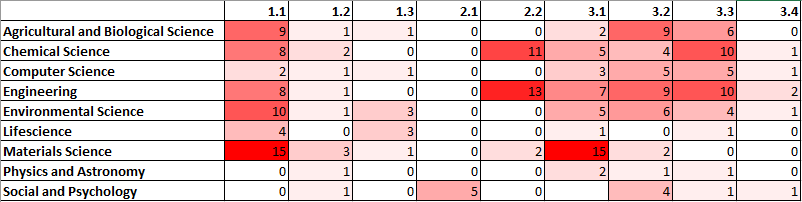
\includegraphics[width=1.0\linewidth]{Heatmap_v4.PNG}
    \caption{Tavoitteiden esiintyvyys eri tieteenaloilla}
    \label{fig:heatmap_v1}
\end{figure}

\begin{table}[ht]
    \centering
    \begin{tabular}{|c|c|}
        \hline
        \textbf{Tieteenala} & \textbf{Lukumäärä} \\
        \hline
        Agricultural and Biological Science & 24 \\
        \hline
        Chemical Science & 30 \\
        \hline
        Computer Science & 14 \\
        \hline
        Engineering & 39 \\
        \hline
        Environmental Science & 29 \\
        \hline
        Lifescience & 7 \\
        \hline
        Materials Science & 27 \\
        \hline
        Physics and Astronomy & 5 \\
        \hline
        Social and Psychology & 9 \\
        \hline
        \textbf{Yhteensä} & \textbf{184} \\
        \hline
    \end{tabular}
    \caption{Löydettyjen tutkimusartikkelien määrät tieteenaloittain}
    \label{tab:tieteenalat lkm}
\end{table}

\section{Löydetyt laadullisten simulaatioiden ohjeet ja työkalut} \label{tyokalut}
Seuraavissa listoissa on esitetty tutkimuksista tunnistetut mallintamisen työkalut 
ja algoritmit sekä tietokoneohjelmat,
joita käytettiin laadullisten simulaatioiden luomisessa ja ajamisessa. 
Nämä ovat jaettu kahteen kategoriaan, mallintamisen työkalut 
ja tietokoneohjelmistot. 
Kategoriaan ''mallintaminen'' kuuluvat metodit ja algoritmit 
joiden avulla ollaan mallinnettu tai suunniteltu laadullisia malleja.
Kategoriaan ''ohjelmistot'' kuuluvat tietokoneohjelmat ja ohjelmistot 
joiden avulla ollaan joko luotu tai ajettu laadullisia simulaatioita.

\subsection{Mallintaminen}
Aineistosta tunnistetut mallintamisen työkalut ja ohjelmistot on jaettu kolmeen
tavoitekategoriaan tieteenaloittain. Taulukossa ensimmäinen sarake merkitsee
tieteenalaa  ja toinen mallintaminen merkitsee löydetyt ja tunnistetut 
mallintamisen metodit ja algoritmit. Kolmas sarake on ohjelmistoille. 
Työkaluihin on suluissa merkitty 
kuinka monta kertaa kyseinen työkalu on esiintynyt eri artikkeleissa.

\begin{longtable}[h]{|p{4cm}|p{6cm}|p{5cm}|}
    \hline
    \textbf{Tieteenala}    &    \textbf{Mallintaminen}  &  \textbf{Ohjelma}\\
    \hline
    Agricultural and Biological Science & 
    \begin{itemize}
        \item discrete element method
    \end{itemize} &
    \begin{itemize}
        \item CompuCell3D
        \item GNA (4)
        \item Idrisi GIS software
        \item OVITO
        \item QTIP - Qualitative Temporal Inference Program
    \end{itemize} 
    \\
    \hline
    Chemical Science & \begin{itemize}
        \item Euler-Euler approach
        \item signed directed graph
    \end{itemize} &
    \begin{itemize}
        \item Chemkin-Pro software
        \item COMSOL software (2)
        \item GROMACS 4.5 software
        \item HyperChem 8.0 software
        \item OpenFOAM (2)
        \item ThermRot software
    \end{itemize} 
    \\
    \hline
    Computer Science & \begin{itemize}
        \item agent-based approach
        \item QSIM
    \end{itemize} &
    \begin{itemize}
        \item Matlab (2)
    \end{itemize} 
    \\
    \hline
    Engineering & \begin{itemize}
        \item fuzzy qualitative simulation algorithm
        \item MARS-KS moving reactor model
        \item Modified Nodal Analysis
        \item variational multiscale method
    \end{itemize} &
    \begin{itemize}
        \item COMSOL software 
        \item FLUENT
        \item Matlab
    \end{itemize}
    \\
    \hline
    Environmental Science & \begin{itemize}
        \item Jacob-Levins community matrix
        \item multi-objective modified seagull optimization algorithm
        \item QSIM (2)
        \item signed digraph
        \item slime mould algorithm
    \end{itemize} &
    \begin{itemize}
        \item EPANET software
        \item Garp3 (6)
        \item GMS-7 software
        \item Matlab (4)
        \item MODFLOW software
        \item ReaDDy 2 software
    \end{itemize}
    \\
    \hline
    Materials Science & \begin{itemize}
        \item lattice Boltzmann method
        \item molecular dynamics
    \end{itemize} & 
    \begin{itemize}
        \item COMSOL software 
        \item DEAL.II
        \item Flow3d
        \item FLUENT (2)
        \item LAMMPS
        \item Materials Studio
        \item Matlab
        \item Pace3D 
    \end{itemize}
    \\
    \hline
    Lifescience & \begin{itemize}
        \item finite element method (3)
    \end{itemize} &
    \begin{itemize}
        \item ANSYS software
        \item Matlab (3)
    \end{itemize}
    \\
    \hline
    Physics and Astronomy & \begin{itemize}
        \item Nose–Hoover dynamics
    \end{itemize} &
    
    \\
    \hline
    \caption{Työkalut ja ohjelmistot, järjestelmän toiminnan kuvaaminen.}
    \label{table:mallintaminen 1.}
\end{longtable}

\pagebreak

\begin{longtable}[h]{|p{4cm}|p{6cm}|p{5cm}|}
    \hline
    \textbf{Tieteenala}    &    \textbf{Mallintaminen} & \textbf{Ohjelma}\\
    \hline
    Chemical Science & \begin{itemize}
        \item fault-tree structures
        \item fuzzy logic (3)
        \item fuzzy set theory
        \item signed digraph
        \item Signed Directed Graph (5)
    \end{itemize} & 
    \begin{itemize}
        \item Matlab (2)
        \item SIMULINK
    \end{itemize}
    \\
    \hline
    Engineering & \begin{itemize}
        \item fault-tree structures
        \item fuzzy inductive reasoning
        \item fuzzy qualitative simulation algorithm (3)
        \item FONM - Functional Ontology for Naive Mechanics 
        \item qualitative fault isolation (QFI) framework
        \item QSIM (2)
        \item Signed Directed Graph (2)
        \item SQMA (Situation-based Qualitative Modeling and Analysis)
    \end{itemize} & 
    \begin{itemize}
        \item Visual-FIR
    \end{itemize}
    \\
    \hline
    Materials Science & \begin{itemize}
        \item discrete element method
    \end{itemize} &
    
    \\
    \hline
    Social and Psychological Sciences & \begin{itemize}
        \item catastrophe theory
        \item fuzzy set theory (2)
        \item GA-BP (Genetic Algorithm – Back Propagation Neural Network Algorithm)
        \item QSIM (4)
    \end{itemize} & 
    \begin{itemize}
        \item AnyLogic
    \end{itemize}
    \\   
    \hline
    \caption{Työkalut ja ohjelmistot, vikatilojen analysointi}
    \label{table:mallintaminen 2.}
\end{longtable}

\begin{longtable}[h]{|p{4cm}|p{6cm}|p{5cm}|}
    \hline
    \textbf{Tieteenala}    &    \textbf{Mallintaminen} & \textbf{Ohjelma}\\
    \hline
    Agricultural and Biological Science & \begin{itemize}
        \item Biomolecular Network Ontology (2)
        \item QSIM
        \item signed digraph
    \end{itemize} &
    \begin{itemize}
        \item GRENS - Gene REgulatory Network Simulator
        \item GINsim - Gene Interaction Network simulation
        \item GNA (3)
        \item Matlab (4)
        \item TAM-B
    \end{itemize} 
    \\
    \hline
    Chemical Science & \begin{itemize}
        \item Cause-Effect matrix
        \item discrete element method
        \item Extended Signed Directed Graph
        \item fault trees
        \item fuzzy set theory
        \item piping and instrumentation diagrams
        \item QSIM
        \item signed digraph
        \item Signed Directed Graph (2)       
        \item state-based approach
    \end{itemize} & 
    \begin{itemize}
        \item Chemkin-Pro software
        \item OpenFOAM
        \item TAM-C
        \item ThermRot software
        \item WINEPR-Simfonia
    \end{itemize}
    \\
    \hline
    Computer Science & \begin{itemize}
        \item agent-based approach
        \item exogenization and equilibration techniques
        \item genetic algorithms
        \item GDE algorithm (2)
        \item Rough Set Theory
        \item Signed Directed Graph
        \item SQMA - Situation-based Qualitative Modeling and Analysis
    \end{itemize} & 
    \begin{itemize}
        \item Garp3 (3)
        \item GNA
        \item LASS (2)
        \item ns-2 simulator
        \item Simulink
    \end{itemize}
    \\
    \hline
    Engineering & \begin{itemize}
        \item Causal Loop Diagrams
        \item Dynamic trend analysis
        \item Fuzzy Inductive Reasoning
        \item fuzzy qualitative simulation algorithm
        \item MARS-KS moving reactor model
        \item QSIM (3)
        \item Qualitative Archi Bond Graphs
        \item qualitative fault isolation (QFI) framework
        \item Signed Directed Graph
        \item situation-operator modeling (SOM) technique
        \item variational multiscale method
    \end{itemize} &
    \begin{itemize}
        \item Matlab
        \item MAGMAS3D
        \item TCAD
        \item Visual-FIR
        \item SABER software (3)
        \item SQSIM software
        \item TAM-C (2)
        \item V-REP
        \item Visual-FIR
    \end{itemize}
    \\
    \hline
    Environmental Science & \begin{itemize}
        \item DEVS formalism
        \item Jacob-Levins community matrix
        \item multi-objective particle swarm optimization algorithm (2)
        \item signed digraph
        \item stochastic social choice rules
    \end{itemize} &
    \begin{itemize}
        \item EcoMata (2)
        \item FLUENT
        \item Garp3
        \item GMS-7 software
        \item Matlab (3)
    \end{itemize}
    \\
    \hline
    Materials Science & \begin{itemize}
        \item elastoplastic coupling constitutive framework
        \item finite-difference time-domain (FDTD) approach
        \item finite element method (2)
        \item form particle difference method
        \item lattice Boltzmann method
    \end{itemize} &
    \begin{itemize}
        \item COMSOL software
        \item DEAL.II 
        \item Maplesoft
        \item Materials Studio
        \item Poynting
        \item SCAPS 1D
        \item TCAD (2)
    \end{itemize}
    \\
    \hline
    Lifescience & \begin{itemize}
        \item QSIM
    \end{itemize} &
    \begin{itemize}
        \item Matlab
    \end{itemize}
    \\
    \hline
    Physics and Astronomy & \begin{itemize}
        \item finite element method
    \end{itemize} &
    
    \\
    \hline
        Social and Psychological Sciences & \begin{itemize}
        \item agent-based approach
        \item GA-BP (Genetic Algorithm – Back Propagation Neural Network Algorithm)
        \item multi-agent qualitative simulation approach
        \item QSIM (2)
    \end{itemize} &
    \begin{itemize}
        \item Presage2
        \item Repast software
        \item SWARM software
    \end{itemize}
    \\
    \hline
    \caption{Työkalut ja ohjelmistot, menetelmäkehitys}
    \label{table:mallintaminen 3.}
\end{longtable}

\subsection{Lyhyet selitykset ohjelmistoista} \label{selitys}
Taulukoissa \ref{table:mallintaminen 1.}, \ref{table:mallintaminen 2.} 
ja \ref{table:mallintaminen 3.} näkyvät vain ohjelmien ja ohjelmistojen nimet.
Tästä alaluvussa on tarkoitus antaa lyhyet selitykset mitä simulaatiotyyppejä 
on toteutettu milläkin simulaatio-ohjelmilla. 

Ohjelmia Repast, SWARM ja Presage2 oltiin käytetty agenttipohjaisten simulaatioiden ajamiseen.
Agenttipohjaisessa simulaatiossa järjestelmän toimintaa mallinetaan itsenäisesti toimivien
agenttien ja niiden vuorovaikutusten kautta.
Ohjelmilla OpenFOAM, FLUENT, GMS-7 ja Flow3D simuloitiin eri nesteiden dynamiikkaa ja toimintaa.
Molekyylien dynamiikkaa simuloitiin ohjelmilla 
LAMMPS, Materials Studio ja GROMACS 4.5.

Jatkuva-aikaisia ja diskreetin elementin laadullisia 
simulaatioita löytyi myös tutkimuksista.
Ohjelmia AnyLogic, Matlab, Maplesoft, WINEPR-Simfonia, SCAPS 1D, Pace3D ja DIOS 
oltiin käytetty eri jatkuva-aikaisten simulaatioiden käyttämisessä.
Diskreetin elementin simulaatioita oltiin toteutettu ohjelmilla
LIGGGHTS, OVITO, ns-2 simulator, Idrisi GIS, SABER, Matlab ja V-REP
\textit{Elementtimenetelmän (eng. Finite element method)} simulaatioita
ajaettiin ohjelmilla, ANSYS, Matlab, COMSOL, Poynting ja DEAL.II.

Geeniverkkojen laadulliseen simulointiin tarkoitettuja ohjelmia ovat
GNA (Genetic Network Analyzer), 
GRENS (Gene REgulatory Network Simulator),
GINsim (Gene Interaction Network simulation) ja CellNetAnalyzer.
Lisäksi myös Matlab-sovellusta oltiin käytetty geeniverkkojen simuloinnissa.

Muita mainittavia simulaatio-ohjelmia, jotka eivät sovi yleisimpiin 
simulaatiotyyppeihin:
\begin{itemize}
    \item Matlab oli käytössä myös ''Signed Directed Graph'' pohjaisissa simulaatioissa.
    \item ReaDDy 2 simulaattorilla simuloitiin partikkelien vuorovaikutusten dynamiikkaa.
    \item Chemkin-Pro ohjelmalla simuloitiin hajoamisreittejä bimolekulaarisissa reaktioissa
    \item HyperChem 8.0 simulaattoria käytettiin molekyylien mekaniikkojen tutkimisessa.
    \item LUX ohjelmaa käytettiin Monte Carlo -pohjaisessa valon säteilyn simuloinnissa.
\end{itemize}

Lisäksi oli useampi ohjelma, jota käytettiin ainoastaan mallin luomisessa.
Ohjelmiin on merkitty suluissa miten niitä ollaan käytetty mallintamisessa:
\begin{itemize}
    \item TAM-B (biologisten järjestelmien reaktioit)
    \item UPPAAL (geenien rekulaariverkkot).
    \item TAM-C (kinetiikan parametrit ja rakenteet)
    \item SIMULINK (kemiantekniikan vikojen leviämisskenaariot).
    \item ThermRot (molekulaarien termodynaamisen ja kineettisten tietojen laskeminen)
    \item EcoMata (ecojärjestelmät ja niiden käyttäytymiset)
    \item MAGMAS3D (yleisten monikerroksisten taso- ja 3D-rakenteiden analysointi)
    \item LASS (mallinnusympäristö maisemien ja maisemakuvioiden luomiseksi sekä analyysiin)
    \item EPANET (vedenjakelujärjestelmän analyysi)
    \item Visual-FIR (sumeaan induktiiviseen päättelyyn (eng. Fuzzy Inductive Reasoning) perustuva monimutkaisten järjestelmien mallintaminen ja simulointi)
    \item SQSIM (simulaattori, joka ennustaa puoli-määrällisiä käyttäytymiskuvauksia puoli-määrällisistä differentiaaliyhtälöistä)
\end{itemize}

\chapter{Tulosten tulkitseminen ja pohdinta} \label{tulkitseminen ja pohdinta}

\section{Laadullisen simulaation tavoitteet}
Laadullinen simulaatio on kattava aihealue, joilta löytyy tutkimuksia monelta eri alalta.
Tässä tutkimuksessa aineiston artikkeleista tunnistettiin 17 
eri ScienceDirectin määrittelemää tieteenalaa, 
jotka tiivistettiin kymmeneksi alaksi taulukkoon 
\ref{fig:heatmap_v1}.
Käytetystä aineistosta löydettiin yhdeksän eri tavoitetta, 
mitä laadullisella simulaatiolla pyrittiin saavuttamaan tutkimuksessa.

Taulukosta \ref{table: tuloksien kategoriat}, voidaan havaita, 
että eniten yksittäisistä tavoitekategoiroista 
laadullisilla simulaatioilla pyrittiin vähentämään tutkittavan 
kohteen tietoisuuden aukkoja (kategoria 1.1.). 
Tämä vastaa hyvin laadullisen simulaation määritelmää
työkaluna, jolla voidaan simuloida järjestelmiä ilman täydellistä tietoa.
Olosuhteiden muutoksien vaikusta ja järjestelmän käyttäytymisen ennustusta
pyrittiin myös tutkimaan laadullisella simulaatioilla jonkin verran.

Kaikista eniten tutkimuksissa on tutkittu menetelmiä (tavoitekategoria 3.).
Tästä voidaan päätellä, että laadullisien simulaatioiden käyttämistä 
tutkitaan usein, oli kyse sitten vanhojen työkalujen parantamisesta tai 
uusien luomisesta. 
Hakukoneita testatessa tehtiin lyhyt vertaus miten laadullisten simulaatioiden suosio on 
muuttunut. Taulukon \ref{table: hakutulokset} mukaan laadullisten simulaatioiden 
suosio on hieman kasvanut viime 20 vuoden aikana. Google Scholarin haun mukaan kasvu on ollut
merkittävämpi kuin ScienceDirectin haun mukaan.
Tämä on mahdollinen syy miksi työkaluja ollaan kehittämässä laadullisille simulaatioille
niin paljon.

Kohdejärjestelmien vikojen tai epätoivottujen toiminnan selvittämistä 
oltiin tutkittu tavoitekategorioista vähiten (tavoitekategoria 2.).
Toteutuneen vian vaikutuksia tutkittiin aika vähän 
verrattuna muihin kategorioihin. 
Ainoat alat missä oltiin kiinnostuneita toteutuneen vian tai haitan vaikutuksesta
oli yhteiskunta ja psykologiset alat. 
Muilla aloilla oltiin selkeästi enemmän kiinnostuneita
vian tai haitan esiintymisen mahdollisuuksista.
Mahdollinen selitys tälle on, että muissa tutkimuksissa, 
jotka liittyivät vikoihin tutkittavissa kohteissa, 
oltiin kiinnostuneempia vian ennaltaehkäisemisestä.

Vertailuja eri työkalujen tehokkuuksien välillä oltiin aika vähän tehty. 
Yksi selitys tälle voi olla, että laadullisen simulaation tutkimuskohteet 
voivat olla liian niukkoja, jotta työkaluja voitaisiin vertailla hyödyllisesti.
On myös mahdollista, että eri laadullisten simulaatioiden työkalujen vertailuja 
löytyy enemmän eri tutkimustietokannista.

\section{Laadullisen simulaation tieteenalat}
Eniten laadullisia simulaatioita aineiston tutkimuksissa
käytettiin kemian tieteen (chemical science),
tekniikan (engineering), ympäristön (environmental) ja materiaalien tieteen  (materials science) tieteenaloilla. 
Vähiten laadullisia simulaatioita käytettiin elämäntieteiden (lifescience),
fysiikan ja astronomian  (Physics and Astronomy) sekä 
yhteiskunnallisten ja psykologisten (Social and Psychology) tieteiden aloilla.
Taulukossa \ref{tab:tieteenalat lkm} näkyvät paljonko mitäkin tieteenalaa
löytyi aineistosta.

Maatalouden ja biologisten (agricultural and biological) tieteiden aloilla
tutkittiin kohdejärjestelmien koskevien tietojen aukkoja ja myös pyrittiin
parantamaan eri laadullisten simulaatioiden työkalujen käyttöä tieteenalan
sisällä.

Kemiantieteissä ja tekniikassa yleisesti 
pyrittiin usein selvittämään kohdejärjestelmässä mahdollisia 
ilmestyviä vikoja tai riskejä.
Näillä aloilla pyrittiin myös usein parantamaan ja 
kehittämään työkaluja laadullisten simulaatioiden käyttöön ja toteuttamiseen.
Tutkimuksissa pyrittiin myös parantamaan tietoisuutta liittyen tutkimuskohteisiin.

Materiaalien tutkimustieteessä pyrittiin selvästi 
tutkimaan materiaaleihin  liittyvistä tietojen ja datan aukkoisuutta, 
ja tutkimuksen laadullisten simulaatioiden tuloksia usein vertailtiin reaalimaailman testeihin ja havaintoihin.

Ympäristötieteissä pyrittiin eniten vähentämään tutkimuskohteiden tietojen aukkoisuuksia, mutta tutkimuksia oli tasaisesti myös jakaantunut tavoitekategorioille 3.1, 3.2 ja 3.4, mikä viittaa siihen, että
metodeja laadullisten simulaatioiden käyttämiseen ja toteutukseen on myös
tutkittu paljon.

Fysiikan ja astronomian aloilla oli erittäin vähän tutkimuksia.
Yksi mahdollinen selitys tälle voi olla,
että usein laadullisesta fysiikasta käytetään termiä ''Qualitative Physics'', jolloinka tutkimuksia voi helposti jäädä aineiston ulkopuolelle.

Yhteiskuntatieteessä (Social Science) löytyi suurimmalta osalta tutkimuksia, 
jotka pyrkivät selvittämään miten mahdollinen haitallinen käyttäytyminen voi vaikuttaa
tilanteeseen. Tämä Voi mahdollisesti johtua Science Directin määritelmistä, esimerkiksi
Päätösteoria (Decision Science) on osittain myös osa yhteiskuntatieteellistä alaa. 
Yksi syy tavoitekategorian 2.1. taulukossa \ref{fig:heatmap_v1}
vähäiselle esiintymiselle voi olla, 
että muilla aloilla ei olla kiinnostuneita haittojen vaikutuksista,
vaan ainoastaan niiden esiintymismahdollisuuksista, 
jos verrataan tavoitekategoriaan 2.2.
Toinen mahdollinen selitys tälle voi olla, 
että ihmisten käyttäytymistä tai toimintaa on vaikea testata ennakkoon valvotussa olosuhteissa, 
joten tapahtumien vaikutusten arviointia on ennakoitava huolellisesti.
Vertauksena taas esimerkiksi tekniikan alalla kiinnostaa se, 
voiko esimerkiksi uusi laiteen prototyyppi toimia. 
Lopulliset testit tehdään prototyypilla ja näin viat tulevat sitä kautta esiin.

\section{Laadullisen simulaation työkalut}
Löydetyistä mallintamisen työkaluista taulukoista \ref{table:mallintaminen 1.},
\ref{table:mallintaminen 2.} ja \ref{table:mallintaminen 3.} voidaan päätellä, 
että QSIM on yleisin käytetty tapa mallintaa laadullisia simulaatioita.
On selkeää, että QSIM on erittäin tunnettu algoritmi ja yksi ensimmäisistä
laadullisille simuloinninlle tarkoitetuista algoritmeista
\parencite{kuipers1986qualitative}.
Mallintamisessa on myös käytetty useita eri abstraktointiin perustuvia sumeita tapoja ja metodeja, kuten alaluvussa \ref{tyokalut} mainittua sumeaa laadullisen simulaation algoritmia.

''Signed Directed graphs'' ja ''signed digraphs'' esiintyivät myös usein, 
varsinkin kemian ja tekniikan tieteenaloilla. Lyhyella katsauksella
metodit ovat käytössä laadullisen simuloinnin, vaara- ja käytettävyysanalysoinnissa 
ja vianselvityksessä \parencite{SDGapplication2004}.
Molemmissa menetelmissä pyritään toteuttamaan syy-seuraus kaavakkeita perustuen
järjestelmän laadullisesti määriteltyyn käyttäytymiseen.

Mallintamisesta löytyy useita eri yksittäisiä metodeja ja algoritmeja. 
Mallintamisessa täytyy tietää tutkittava kohdejärjestelmä hyvin tarkasti, 
jotta toimivaa mallia pystyttäisiin luomaan. Tästä johtuen havainnot 
mallintamisen metodeista ja algoritmeista ei ole niin tärkeä, sillä
mallintamiseen ei ole yleistä, kaikkeen toimivaa tapaa.

Taulukoista \ref{table:mallintaminen 1.}, \ref{table:mallintaminen 2.} ja 
\ref{table:mallintaminen 3.} löytyvät aineiston tutkimuksista löydetyt 
laadullisiin simulaatioihin liittyvät ohjelmistot ja ohjelmat.
Ohjelmistoissa yleisiä ovat Matlab, GNA, Garp3, COMSOL ja OpenFOAM. 
Näistä Matlab esiintyi useimmiten eri tieteenaloilla ja tavoitekategorioissa.

Matlab on erittäin yleinen ohjelma laadullisille simulaatioille, joka esiintyy eri 
tieteenaloissa ja tavoitteissa. Matlab on ohjelmoinnin ja numeerinen laskennan alusta
\footnote{\url{https://se.mathworks.com/products/matlab.html}},
joka on kyvyiltään erittäin monipuolinen, mikä näkyy sen levinneisyydessä. 
Tämä on paikkansa pitävä myös mitä tulee laadullisten simulaatioiden käytölle.

GNA (Genetic Networ Analyzer) on tietokonetyökalu geeniverkkojen mallintamiseen 
ja simulointiin 
\footnote{\url{https://team.inria.fr/microcosme/genetic-network-analyzer-gna/}}. 
Geeniverkkoihin liitty suuri määrä matematiista dataa, mikä tekee niistä vaikeita 
simuloida määrällisesti \parencite{gnaGeneticNetworkAnalyzer2003}, miksikä
GNA on suunniteltu laadulliseen mallintamiseen ja simulointiin. GNA-ohjelmaa 
usein käytettiin maatalouden ja biologisten tieteiden tutkimuksissa.
Muita geeniverkkoihin liittyviä ohjelmistoja on esimerkiksi GINsim ja GRENS,
jotka esiintyvät taulukossa \ref{table:mallintaminen 3.}.

Garp3 
\footnote{\url{https://ivi.fnwi.uva.nl/tcs/QRgroup/QRM/help/faq/index.html\#Software}} 
on ohjelmisto laadullisten mallien tarkastelemiseen, kehittämiseen ja 
ajamiseen. Garp3 on uudempi versio GARP-ohjelmasta, jonka ilmentyminen
yhdistettiin taulukoissa.
Garp3 ja aikaisempi versio GARP olivat eniten käytössä
ympäristötieteen aloilla.

Ohjelmistoissa esiintyy enemmän yhtäläisyyksia eri työkalujen käytössa verrattuna
mallintamisen työkaluihin. Tämä voi johtua siitä, että simulaatio-ohjelman
valitseminen on vähemmän kriittistä kuin mallin luominen. 
Kun on malli saatu luotua, simulaation ajamiselle löytyy yleiskäyttöisiä 
työkaluja, kuten Matlab.

Alaluvussa \ref{selitys} kerrottiin lyhyesti minkä tyyppisiä 
simulaatioita ohjelmistoilla 
toteutettiin. Näistä laadulliseen simulointiin ensisijaisesti tarkoittettuja
menetelmiä ovat QSIM, sumeat algoritmit ja Garp3, mitkä todettiin yleisiksi
menetelmiksi jo ennen kartoituksen toteuttamista. Näistä avattiin enemmän 
alaluvussa \ref{yleiset menetelmat}.

\section{Vastaukset tutkimuskysymyksiin}
Kysymykseen 
''Millaisia tuloksia laadullisilla simulaatioilla pyritään hakemaan?''
vastauksena aineistosta on tunnistettu 9 eri yhtenevää tavoitetta, 
mitä laadullisilla simulaatioilla on pyritty hakemaan. Nämä tavoitteet
koostuvat järjestelmän toiminnan tutkimisesta, 
vikojen ja haittojen selvityksestä ja laadullisten simulaatioiden menetelmien kehittämisestä.

Toinen tutkimuskysymys oli
''Minkä alan tutkimuksissa on eniten käytetty laadullisia simulaatioita?''.
Tähän kysymykseen aineistosta löydettiin 17 eri ScienceDirectin määrittelemää
tieteenalaa, jotka tiivistettiin 9 koostumukseen alaluvussa \ref{tieteenalat}.
Aineistossa aloista eniten esiintyivät tekniikan, kemian tieteiden, ympäristötieteiden ja materiaalitieteiden alat.

Viimeinen tutkimuskysymys oli, että
''Mitä eri työkaluja löytyy laadullisten simulaatioiden luomiseen?''
Tätä varten artikkeleista kerättiin nimetyt laadullisiin simulaatioihin liittyvät
metodit, algoritmit ja ohjelmistot taulukkoihin \ref{table:mallintaminen 1.},
\ref{table:mallintaminen 2.} ja \ref{table:mallintaminen 3.}. 
Näistä useimmin esiintyneet mallintamisen työkalut
ovat QSIM-algoritmi, ''Signed Directed Graph'' ja ''Signed Digraph'' mallit
ja eri sumeaan teoriaan perustuvat menetelmät.
Ohjelmistoista yleisimmät ovat Matlab, GNA ja Garp3 sovellukset.

\section{Tutkimuksen huomiot ja jatkotutkimusehdotukset}
Kartoituksen tieteenaloihin luottaminen tarvitsee sen, 
että luotetaan ScienceDirectin  ja tekoälyn määritelmiin. 
Näistä voidaan kuitenkin luoda alustavia päätelmiä, mutta tarkempia
toteamuksia varten pitäisi laajentaa aineiston hakua useammalle eri tietokannalle ja hakukoneelle. Myös haun tarkentaminen voi parantaa tuloksia, sillä tälle 
aineistolle piti tehdä paljon manuaalista karsimista, 
vaikka käytettiin vain yhtä tutkimustietokantaa.

ScienceDirectin tieteenalojen luokitukset ovat aika laajoja, jotta niihin voitaisiin täydellisesti luottaa. Esim. ''Agricultural and Biological'' ja ''Engineering''. Myös se, että tutkimus voi olla useaa tieteenalaa samaan aikaan täytyy ottaa huomioon mahdollisessa jatkotutkimuksessa. 
Tässä tutkimuksessa pyrittiin rajoittamaan tieteenaloja yksi per artikkeli.

Mahdollisia kyseenalaistavia kysymyksiä tulosten tarkkuudesta ovat seuraavat:
\begin{itemize}
    \item Muuttaako useamman hakukoneen tai tutkimustietokannan käyttäminen näitä tuloksia? 
    \item Voiko aikavälin rajaaminen haussa muuttaa tuloksia? Taulukosta \ref{table: hakutulokset} Nähdään, että laadullisten simulaatioiden suosio on hieman kasvanut
    viimevuosina, mutta ovatko aikavälien sisäiset trendit muuttuneet?
\end{itemize}

Tietokannan hakuun olisi voinut lisätä hakusanoiksi 
''Qualitative Reasoning'' ja ''Qualitative Physics'' OR-ehdolla. 
Näiden termien suureen esiintymismäärään törmättiin vasta aineiston 
analyysin vaiheessa ja olisi vaatinut lisäaikaa tutkimuksen tekemiselle.

Mahdollisia jatkotutkimuskohteita ovat: 
\begin{itemize}
    \item Kirjallisuuskartoituksen parantaminen, kuten laajempi haku ja tieteenalojen tarkempi kategorisointi.
    \item Mahdollisemmat syvällisemmät kirjallisuuskatsaukset eri tieteenaloihin ja työkaluihin.
\end{itemize}

\chapter{Yhteenveto}
Tässä tutkimuksessa pyrittiin selvittämään, miten laadullisia simulaatioita 
käytetään ja toteutetaan tieteellisenä menetelmänä. 
Tutkimuksen keskeiset kysymykset olivat: 
mitä tavoitteita laadullisilla simulaatioilla pyrittiin saavuttamaan, 
millä aloilla simulaatioita hyödynnettiin eniten 
sekä millä työkaluilla simulaatioita toteutettiin. 
Kirjoitusvaiheessa vastaavaa tutkimusta ei ollut saatavilla.

Tutkimuksen menetelmäksi valittiin systemaattinen kirjallisuuskartoitus, koska
menetelmä on sopiva kun halutaan saada pinnallinen katsaus laajaan aihealueeseen.
laadullisten simulaatioiden käytöstä tieteellisenä tutkimusmenetelmänä.
Koska laadulliset simulaatioit olivat aiheena odotettua suurempi, 
kartoituksessa aineiston keruu jouduttiin rajoittamaan ScienceDirectin 
tutkimustietokantaan. Aineistoa haettiin hakutermillä ''Qualitative simulation''
vuosilta 2000-2024. Sopivia artikkeleita valittiin lopuksi yhteensä 184 kappaletta.

Systemaattisen kirjallisuuskartoituksen tuloksena saatiin pinnallinen katsaus miten 
laadulliset simulaatioit ovat käytössä eri tieteenaloilla. 
Laadullisia simulaatioita oltiin eniten käytetty kemian tieteiden, 
tekniikan ja ympäristötieteiden aloilla. Tutkimuksia löytyi kiitettävästi myös
maatalouden ja biologian, sekä energian ja tietotekniikan aloilla. 
Vähiten tutkimuksia löytyi yhteiskunnan ja psykologisten tieteiden aloista, sekä 
fysikaan ja astronomian aloilta.

Eniten laadullisilla simulaatioilla pyrittiin
selvittämään enemmän kohdejärjestelmän toiminnasta, eli korjaamaan tietoisuuden aukkoja
tutkittavasta kohteesta. Viimeisenä 20 vuotena on myös tehty paljon tutkimuksia liittyen 
laadullisten simulaatioiden toteuttamiseen eri aloilla. 
Esimerkiksi uusia työkaluja ollaan kehitetty ja vanhoja paranneltu.
Osittain laadullisilla simulaatioilla on myös pyritty ennustamaan mahdollisia vian 
ilmentymiä, varsinkin kemian tieteiden ja tekniikan aloilla.

Laadullisille simulaatioille löydettiin myös useita eri metodeja ja algoritmeja 
mitä tulee mallintamiseen. Mallintamisen työkalujen valinta on erittäin tärkeää,
jos sopivia työkaluja edes on olemassa. Tästä huolimatta mallintamisen työkaluista
nousivat esille QSIM-algoritmi ja Signed Directed Graph sekä Signed Digraph -kaaviot, 
jotka esiintyivät useammin verrattuna muihin työkaluihin.
Simulaatio-ohjelman valitseminen on selvästi vähemmän kriittistä, sillä ohjelmien taulukoissa
oli selkeästi vähemmän yksittäisiä ohjelmia. 
Yleisin simulaatio-ohjelma on Matlab, mikä johtuu sen monikäyttöisyydestä 
matemaattisena työkaluna.

Toteutettu kirjallisuuskartoitus ei ole kuitenkaan täysin kattava. 
Kartoitus rajoittui resurssien puitteissa ainoastaan yhteen tutkimustietokantaan,
ScienceDirectiin, mikä on otettava huomioon tulosten tulkinnassa. 
Mahdollisia jatkotutkimusehdotuksia ovat kirjallisuuskartoituksen parantaminen, 
johon sisältyisi useamman eri hakukoneen ja tietokannan hyödyntäminen.
Lisäksi jos halutaan syvällisempää tietoa laadullisten simulaatioiden käytöstä, 
voidaan mahdollisesti toteuttaa tarkempia kirjallisuuskatsauksia esimerkiksi yhteen 
tieteenalaan kerrallaan.

\printbibliography

\appendix
\section{Aineistossa käytetyt tutkimukset}

Abdul-Wahab, S A, A Elkamel, M A Al-Weshahi, and A S al Yahmadi. 2007. “Troubleshooting the Brine Heater of the MSF Plant Fuzzy Logic-Based Expert System.” Desalination 217 (1): 100–117. https://doi.org/https://doi.org/10.1016/j.desal.2007.01.014.

Ahmad, Jamil, Jérémie Bourdon, Damien Eveillard, Jonathan Fromentin, Olivier Roux, 
and Christine Sinoquet. 2009. 
“Temporal Constraints of a Gene Regulatory Network: 
Refining a Qualitative Simulation.” Biosystems 98 (3): 149–59.
https://doi.org/https://doi.org/10.1016/j.biosystems.2009.05.002.

Aichernig, Bernhard K, Harald Brandl, and Franz Wotawa. 2009. “Conformance Testing of Hybrid Systems with Qualitative Reasoning Models.” Electronic Notes in Theoretical Computer Science 253 (2): 53–69. https://doi.org/https://doi.org/10.1016/j.entcs.2009.09.051.

Argani, L P, D Misseroni, A Piccolroaz, Z Vinco, D Capuani, and D Bigoni. 2016. “Plastically-Driven Variation of Elastic Stiffness in Green Bodies during Powder Compaction: Part I. Experiments and Elastoplastic Coupling.” Journal of the European Ceramic Society 36 (9): 2159–67. https://doi.org/https://doi.org/10.1016/j.jeurceramsoc.2016.02.012.

Aristov, V v, A A Frolova, S A Zabelok, R R Arslanbekov, and V I Kolobov. 2012. “Simulations of Pressure-Driven Flows through Channels and Pipes with Unified Flow Solver.” Vacuum 86 (11): 1717–24. https://doi.org/https://doi.org/10.1016/j.vacuum.2012.02.043.

Arroyo, Esteban, Mario Hoernicke, Pablo Rodríguez, and Alexander Fay. 2016. “Automatic Derivation of Qualitative Plant Simulation Models from Legacy Piping and Instrumentation Diagrams.” Computers \& Chemical Engineering 92: 112–32. https://doi.org/https://doi.org/10.1016/j.compchemeng.2016.04.040.

Ayadi, Ali, Cecilia Zanni-Merk, François de Bertrand de Beuvron, Julie Thompson, and Saoussen Krichen. 2019. “BNO—An Ontology for Understanding the Transittability of Complex Biomolecular Networks.” Journal of Web Semantics 57: 100495. https://doi.org/https://doi.org/10.1016/j.websem.2019.01.002.

Baldazzi, Valentina, Delphine Ropers, Johannes Geiselmann, Daniel Kahn, and Hidde de Jong. 2012. “Importance of Metabolic Coupling for the Dynamics of Gene Expression Following a Diauxic Shift in Escherichia Coli.” Journal of Theoretical Biology 295: 100–115. https://doi.org/https://doi.org/10.1016/j.jtbi.2011.11.010.

Barbari, Matteo, Alberto Cavalli, Lorenzo Fiorineschi, Massimo Monti, and Marco Togni. 2014. “Innovative Connection in Wooden Trusses.” Construction and Building Materials 66: 654–63. https://doi.org/https://doi.org/10.1016/j.conbuildmat.2014.06.022.

Barnat, J, L Brim, I Černá, S Dražan, J Fabriková, and D Šafránek. 2009. “On Algorithmic Analysis of Transcriptional Regulation by LTL Model Checking.” Theoretical Computer Science 410 (33): 3128–48. https://doi.org/https://doi.org/10.1016/j.tcs.2009.02.017.

Barnat, J, L Brim, I Černá, S Dražan, and D Šafránek. 2008. “Parallel Model Checking Large-Scale Genetic Regulatory Networks with DiVinE.” Electronic Notes in Theoretical Computer Science 194 (3): 35–50. https://doi.org/https://doi.org/10.1016/j.entcs.2007.12.001.

Bellazzi, R, R Guglielmann, and L Ironi. 2001. “Learning from Biomedical Time Series through the Integration of Qualitative Models and Fuzzy Systems.” Artificial Intelligence in Medicine 21 (1): 215–20. https://doi.org/https://doi.org/10.1016/S0933-3657(00)00088-9.

Bellazzi, Riccardo, Raffaella Guglielmann, Liliana Ironi, and Cesare Patrini. 2001. “A Hybrid Input-Output Approach to Model Metabolic Systems: An Application to Intracellular Thiamine Kinetics.” Journal of Biomedical Informatics 34 (4): 221–48. https://doi.org/https://doi.org/10.1006/jbin.2001.1022.

Bernard, Olivier, and Jean-Luc Gouzé. 2002. “Global Qualitative Description of a Class of Nonlinear Dynamical Systems.” Artificial Intelligence 136 (1): 29–59. https://doi.org/https://doi.org/10.1016/S0004-3702(01)00169-2.

Bourgeat, Johan, and Philippe Galy. 2013. “Single and Compact ESD Device Beta-Matrix Solution Based on Bidirectional SCR Network in Advanced 28/32 Nm Technology Node.” Solid-State Electronics 87: 34–42. https://doi.org/https://doi.org/10.1016/j.sse.2013.04.033.

Brown, Alexander L, and Walter F Dabberdt. 2003. “Modeling Ventilation and Dispersion for Covered Roadways.” Journal of Wind Engineering and Industrial Aerodynamics 91 (5): 593–608. https://doi.org/https://doi.org/10.1016/S0167-6105(02)00472-5.

Bulitko, Vadim, and David C Wilkins. 2003. “Qualitative Simulation of Temporal Concurrent Processes Using Time Interval Petri Nets.” Artificial Intelligence 144 (1): 95–124. https://doi.org/https://doi.org/10.1016/S0004-3702(02)00369-7.

Calado, J M F, F.P.N.F. Carreira, M.J.G.C. Mendes, J M G Sá da Costa, and M Bartys. 2003. “Fault Detection Approach Based on Fuzzy Qualitative Reasoning Applied to the DAMADICS Benchmark Problem.” IFAC Proceedings Volumes 36 (5): 1077–82. https://doi.org/https://doi.org/10.1016/S1474-6670(17)36636-3.

Calado, J M F, J M G Sá da Costa, M Bartys, and J Korbicz. 2006. “FDI Approach to the DAMADICS Benchmark Problem Based on Qualitative Reasoning Coupled with Fuzzy Neural Networks.” Control Engineering Practice 14 (6): 685–98. https://doi.org/https://doi.org/10.1016/j.conengprac.2005.03.025.

Canale, Giacomo, Felice Rubino, and Roberto Citarella. 2024. “Design Aspects of a CMC Coating-like System for Hot Surfaces of Aero Engine Components.” Forces in Mechanics 14: 100251. https://doi.org/https://doi.org/10.1016/j.finmec.2023.100251.

Cao, Qinggui, Kai Yu, Lujie Zhou, Linlin Wang, and Chunai Li. 2019. “In-Depth Research on Qualitative Simulation of Coal Miners’ Group Safety Behaviors.” Safety Science 113: 210–32. https://doi.org/https://doi.org/10.1016/j.ssci.2018.11.012.

Chan, H Y, M P Srinivasan, F Benistant, K R Mok, Lap Chan, and H M Jin. 2006. “Continuum Modeling of Post-Implantation Damage and the Effective plus Factor in Crystalline Silicon at Room Temperature.” Thin Solid Films 504 (1): 269–73. https://doi.org/https://doi.org/10.1016/j.tsf.2005.09.167.

Chang, Chuei-Tin, and Jung-Yang Chen. 2009. “Systematic Development of Automata Generated Languages for Fault Diagnosis in Continuous Chemical Processes.” IFAC Proceedings Volumes 42 (11): 303–8. https://doi.org/https://doi.org/10.3182/20090712-4-TR-2008.00047.

Chang, Sheng-Yung, Cheng-Ren Lin, and Chuei-Tin Chang. 2002. “A Fuzzy Diagnosis Approach Using Dynamic Fault Trees.” Chemical Engineering Science 57 (15): 2971–85. https://doi.org/https://doi.org/10.1016/S0009-2509(02)00178-1.

Chen, Jung Yang, and Chuei-Tin Chang. 2009. “Development of Fault Diagnosis Strategies Based on Qualitative Predictions of Symptom Evolution Behaviors.” Journal of Process Control 19 (5): 842–58. https://doi.org/https://doi.org/10.1016/j.jprocont.2008.11.006.

Chen, Tao, Xiaoke Ku, Jianzhong Lin, and Hanhui Jin. 2019. “Modelling the Combustion of Thermally Thick Biomass Particles.” Powder Technology 353: 110–24. https://doi.org/https://doi.org/10.1016/j.powtec.2019.05.011.

Chen, Wei, Jianyong Zhang, Timothy Donohue, Kenneth Williams, Ruixue Cheng, Mark Jones, and Bin Zhou. 2017. “Effect of Particle Degradation on Electrostatic Sensor Measurements and Flow Characteristics in Dilute Pneumatic Conveying.” Particuology 33: 73–79. https://doi.org/https://doi.org/10.1016/j.partic.2016.10.004.

Chen, Zhiyuan, and Tiemin Li. 2023. “Precise Geometry and Pose Measurement of In-Hand Objects with Simple Features Using a Multi-Camera System.” Manufacturing Letters 35: 40–48. https://doi.org/https://doi.org/10.1016/j.mfglet.2023.07.020.

Chipaux, R, and M Géléoc. 2000. “Modelisation and Simulation of the Light Collection in the CMS Lead Tungstate Crystals.” Nuclear Instruments and Methods in Physics Research Section A: Accelerators, Spectrometers, Detectors and Associated Equipment 451 (3): 610–22. https://doi.org/https://doi.org/10.1016/S0168-9002(00)00334-X.

Cui, Yunqiu, Chunjie Niu, Jianhua Lv, Hongyu Fan, Chao Chen, Dongping Liu, Na Lu, Guangjiu Lei, and Weiyuan Ni. 2023. “Temperature Dependence of Surface Microstructure of 316 L Stainless Steel Exposed to Low-Energy Hydrogen Ion Irradiation.” Fusion Engineering and Design 196: 113976. https://doi.org/https://doi.org/10.1016/j.fusengdes.2023.113976.

Dafalias, Yannis F, and Majid T Manzari. 2024. “Rate Dependent but Time Independent Plasticity Formulation with Application to Sand.” Mechanics Research Communications 135: 104242. https://doi.org/https://doi.org/10.1016/j.mechrescom.2023.104242.

Daigle, Matthew J, Anibal Bregon, Xenofon Koutsoukos, Gautam Biswas, and Belarmino Pulido. 2016. “A Qualitative Event-Based Approach to Multiple Fault Diagnosis in Continuous Systems Using Structural Model Decomposition.” Engineering Applications of Artificial Intelligence 53: 190–206. https://doi.org/https://doi.org/10.1016/j.engappai.2016.04.002.

Davidsson, Paul, and Magnus Boman. 2005. “Distributed Monitoring and Control of Office Buildings by Embedded Agents.” Information Sciences 171 (4): 293–307. https://doi.org/https://doi.org/10.1016/j.ins.2004.09.007.

Dias, R I, P Salles, and R H Macedo. 2009. “Mate Guarding and Searching for Extra-Pair Copulations: Decision-Making When Interests Diverge.” Ecological Informatics 4 (5): 405–12. https://doi.org/https://doi.org/10.1016/j.ecoinf.2009.09.008.

Dou, Liangtan, Ying Sun, and Lian She. 2012. “Research on Efficiency of Collaborative Allocation System of Emergency Material Based on Synergetic Theory.” Systems Engineering Procedia 5: 240–47. https://doi.org/https://doi.org/10.1016/j.sepro.2012.04.038.

Drăgoicea, Monica, João Falcão e Cunha, and Monica Pătraşcu. 2015. “Self-Organising Socio-Technical Description in Service Systems for Supporting Smart User Decisions in Public Transport.” Expert Systems with Applications 42 (17): 6329–41. https://doi.org/https://doi.org/10.1016/j.eswa.2015.04.029.

Dubi, Shay, Chen Dubi, and Yonatan Dubi. 2007. “A Two Phase Harmonic Model for Left Ventricular Function.” Medical Engineering \& Physics 29 (9): 984–88. https://doi.org/https://doi.org/10.1016/j.medengphy.2006.10.015.

Edwards, Roderick, and Liliana Ironi. 2014. “Periodic Solutions of Gene Networks with Steep Sigmoidal Regulatory Functions.” Physica D: Nonlinear Phenomena 282 (July): 1–15. https://doi.org/10.1016/J.PHYSD.2014.04.013.

Eggeman, A S, A London, and P A Midgley. 2013. “Ultrafast Electron Diffraction Pattern Simulations Using GPU Technology. Applications to Lattice Vibrations.” Ultramicroscopy 134: 44–47. https://doi.org/https://doi.org/10.1016/j.ultramic.2013.05.013.

Eisenack, K, and J Kropp. 2001. “Assessment of Management Options in Marine Fisheries by Qualitative Modelling Techniques.” Marine Pollution Bulletin 43 (7): 215–24. https://doi.org/https://doi.org/10.1016/S0025-326X(01)00076-5.

Eisenack, K, H Welsch, and J P Kropp. 2006. “A Qualitative Dynamical Modelling Approach to Capital Accumulation in Unregulated Fisheries.” Journal of Economic Dynamics and Control 30 (12): 2613–36. https://doi.org/https://doi.org/10.1016/j.jedc.2005.08.004.

Escobet, Antoni, Àngela Nebot, and Francisco Mugica. 2014. “PEM Fuel Cell Fault Diagnosis via a Hybrid Methodology Based on Fuzzy and Pattern Recognition Techniques.” Engineering Applications of Artificial Intelligence 36: 40–53. https://doi.org/https://doi.org/10.1016/j.engappai.2014.07.008.

Eskandaripour, Mehrtash, Mohammad H Golmohammadi, and Shahrokh Soltaninia. 2023. “Optimization of Low-Impact Development Facilities in Urban Areas Using Slime Mould Algorithm.” Sustainable Cities and Society 93: 104508. https://doi.org/https://doi.org/10.1016/j.scs.2023.104508.

Eskandaripour, Mehrtash, and Shahrokh Soltaninia. 2024. “Optimal Low-Impact Development Facility Design in Urban Environments: A Multidimensional Optimization Approach Employing Slime Mould and Nondominated Sorting Genetic Algorithms.” Urban Climate 55: 101963. https://doi.org/https://doi.org/10.1016/j.uclim.2024.101963.

Evdochenko, E, A Kalde, J di Ronco, K Albert, J Kamp, and Matthias Wessling. 2024. “Unraveling the Ion Transport through Top and Wall Coated Polyelectrolyte Membrane Pores.” Desalination, 118170. https://doi.org/https://doi.org/10.1016/j.desal.2024.118170.

Fan, Guo-Wei, and Xue-Feng Li. 2024. “Hypoplastic Constitutive Model of Inherently Anisotropic Sand.” Computers and Geotechnics 175: 106645. https://doi.org/https://doi.org/10.1016/j.compgeo.2024.106645.

Feng, Yahui, Hongxia Guo, Wuying Ma, Jiawen Hu, Xiaoping Ouyang, Jinxin Zhang, Fengqi Zhang, et al. 2024. “Effect of 60Coγ Ray Radiation on Electrical Properties of SiGe HBTs at Low Temperatures.” Microelectronics Journal 144: 106058. https://doi.org/https://doi.org/10.1016/j.mejo.2023.106058.

Fernandes, Eduarda, Irene López-Sicilia, Maria Teresa Martín-Romero, Juan Giner-Casares, and Marlene Lúcio. 2024. “A Stratum Corneum Lipid Model as a Platform for Biophysical Profiling of Bioactive Chemical Interactions at the Skin Level.” Journal of Molecular Liquids 400: 124513. https://doi.org/https://doi.org/10.1016/j.molliq.2024.124513.

Galuza, A, I Kolenov, D Vinnikov, S Mizrakhy, and A Savchenko. 2022. “Investigation of Micro-Arc Oxidation Coatings Using Sub-THz Ellipsometry.” Materials Characterization 189: 111930. https://doi.org/https://doi.org/10.1016/j.matchar.2022.111930.

GAO, Dong, Chongguang WU, Beike ZHANG, and Xin MA. 2010. “Signed Directed Graph and Qualitative Trend Analysis Based Fault Diagnosis in Chemical Industry.” Chinese Journal of Chemical Engineering 18 (2): 265–76. https://doi.org/https://doi.org/10.1016/S1004-9541(08)60352-3.

Gelman, Irit Askira. 2005. “Addressing Time-Scale Differences among Decision-Makers through Model Abstractions.” European Journal of Operational Research 160 (2): 325–35. https://doi.org/https://doi.org/10.1016/j.ejor.2003.09.004.

Ghafari, Sara, Mohammad Ebrahim Banihabib, and Saman Javadi. 2020. “A Framework to Assess the Impact of a Hydraulic Removing System of Contaminate Infiltration from a River into an Aquifer (Case Study: Semnan Aquifer).” Groundwater for Sustainable Development 10: 100301. https://doi.org/https://doi.org/10.1016/j.gsd.2019.100301.

Ghasemi, M A, and S R Falahatgar. 2020. “Qualitative Description on Channel Cracking in Ceramic Type Coatings Due to Substrate Tension Using 3D Discrete Element Method.” Ceramics International 46 (5): 5548–65. https://doi.org/https://doi.org/10.1016/j.ceramint.2019.08.198.

Goethem, S van, J.-M. Jacquet, L Brim, and D Šafránek. 2013. “Timed Modelling of Gene Networks with Arbitrarily Precise Expression Discretization.” Electronic Notes in Theoretical Computer Science 293: 67–81. https://doi.org/https://doi.org/10.1016/j.entcs.2013.02.019.

Goulart, Fernando F, Paulo Salles, Carlos H Saito, and Ricardo B Machado. 2013. “How Do Different Agricultural Management Strategies Affect Bird Communities Inhabiting a Savanna-Forest Mosaic? A Qualitative Reasoning Approach.” Agriculture, Ecosystems \& Environment 164: 114–30. https://doi.org/https://doi.org/10.1016/j.agee.2012.09.011.

Guerrin, F, and J Dumas. 2001. “Knowledge Representation and Qualitative Simulation of Salmon Redd Functioning. Part II: Qualitative Model of Redds.” Biosystems 59 (2): 85–108. https://doi.org/https://doi.org/10.1016/S0303-2647(01)00101-0.

Guerrin, François, and Jacques Dumas. 2001. “Knowledge Representation and Qualitative Simulation of Salmon Redd Functioning. Part I: Qualitative Modeling and Simulation.” Biosystems 59 (2): 75–84. https://doi.org/https://doi.org/10.1016/S0303-2647(01)00100-9.

Gueven, A, and Z Hicsasmaz. 2011. “Geometric Network Simulation of High Porosity Foods.” Applied Mathematical Modelling 35 (10): 4824–40. https://doi.org/https://doi.org/10.1016/j.apm.2011.03.047.

Gutiérrez, M A, H Khanbareh, and S van der Zwaag. 2016. “Computational Modeling of Structure Formation during Dielectrophoresis in Particulate Composites.” Computational Materials Science 112: 139–46. https://doi.org/https://doi.org/10.1016/j.commatsci.2015.10.011.

Hamagchi, Takashi, Yoshihiro Hashimoto, Toshiaki Itoh, Akihiko Yoneya, and Yoshitaka Togari. 2001. “Abnormal Situation Correction Based on Cascade/Ratio Control.” IFAC Proceedings Volumes 34 (27): 209–14. https://doi.org/https://doi.org/10.1016/S1474-6670(17)33593-0.

Hasan, Salim Ibrahim, Serhan Küçüka, and Mehmet Akif Ezan. 2023. “Cooling Performance of a Piezo-Fan Oscillating in a Vertical Channel with Natural Convection.” International Communications in Heat and Mass Transfer 141: 106602. https://doi.org/https://doi.org/10.1016/j.icheatmasstransfer.2022.106602.

Honorien, J, R Fournet, P.-A. Glaude, and B Sirjean. 2021. “Theoretical Study of the Gas-Phase Thermal Decomposition of Urea.” Proceedings of the Combustion Institute 38 (1): 355–64. https://doi.org/https://doi.org/10.1016/j.proci.2020.06.012.

Hu, Bin, and Ni Xia. 2015a. “Cusp Catastrophe Model for Sudden Changes in a Person’s Behavior.” Information Sciences 294: 489–512. https://doi.org/https://doi.org/10.1016/j.ins.2014.09.055.

———. 2015b. “Cusp Catastrophe Model for Sudden Changes in a Person’s Behavior.” Information Sciences 294 (February): 489–512. https://doi.org/10.1016/J.INS.2014.09.055.

Hussain, Raja Rizwan, and Tetsuya Ishida. 2009. “Critical Carbonation Depth for Initiation of Steel Corrosion in Fully Carbonated Concrete and Development of Electrochemical Carbonation Induced Corrosion Model.” International Journal of Electrochemical Science 4 (8): 1178–95. https://doi.org/https://doi.org/10.1016/S1452-3981(23)15216-3.

Ironi, Liliana, and Diana X Tran. 2016. “Nonlinear and Temporal Multiscale Dynamics of Gene Regulatory Networks: A Qualitative Simulator.” Mathematics and Computers in Simulation 125: 15–37. https://doi.org/https://doi.org/10.1016/j.matcom.2015.11.007.

Jagannathan, N Suhas, and Lisa Tucker-Kellogg. 2016. “Membrane Permeability during Pressure Ulcer Formation: A Computational Model of Dynamic Competition between Cytoskeletal Damage and Repair.” Journal of Biomechanics 49 (8): 1311–20. https://doi.org/https://doi.org/10.1016/j.jbiomech.2015.12.022.

Jong, Hidde de, Johannes Geiselmann, Grégory Batt, Céline Hernandez, and Michel Page. 2004. “Qualitative Simulation of the Initiation of Sporulation in Bacillus Subtilis.” Bulletin of Mathematical Biology 66 (2): 261–99. https://doi.org/https://doi.org/10.1016/j.bulm.2003.08.009.

Jong, Hidde de, Jean Luc Gouzé, Céline Hernandez, Michel Page, Tewfik Sari, and Johannes Geiselmann. 2004. “Qualitative Simulation of Genetic Regulatory Networks Using Piecewise-Linear Models.” Bulletin of Mathematical Biology 66 (2): 301–40. https://doi.org/10.1016/J.BULM.2003.08.010.

Ju, Shi-Ning, Cheng-Liang Chen, and Chuei-Tin Chang. 2003. “Fault-Tree Structures of Override Control Systems.” Reliability Engineering \& System Safety 81 (2): 163–81. https://doi.org/https://doi.org/10.1016/S0951-8320(03)00086-3.

Junior, Flávio Neves, and Joseph Aguilar Martin. 2000. “Heterogeneous Control and Qualitative Supervision, Application to a Distillation Column.” Engineering Applications of Artificial Intelligence 13 (2): 179–97. https://doi.org/https://doi.org/10.1016/S0952-1976(99)00051-2.

Jurado, Sergio, Àngela Nebot, Fransisco Mugica, and Narcís Avellana. 2015. “Hybrid Methodologies for Electricity Load Forecasting: Entropy-Based Feature Selection with Machine Learning and Soft Computing Techniques.” Energy 86: 276–91. https://doi.org/https://doi.org/10.1016/j.energy.2015.04.039.

Kansou, Kamal, and Bert Bredeweg. 2014. “Hypothesis Assessment with Qualitative Reasoning: Modelling the Fontestorbes Fountain.” Ecological Informatics 19: 71–89. https://doi.org/https://doi.org/10.1016/j.ecoinf.2013.10.007.

Karunasena, H C P, Y T Gu, R J Brown, and W Senadeera. 2015. “Numerical Investigation of Plant Tissue Porosity and Its Influence on Cellular Level Shrinkage during Drying.” Biosystems Engineering 132: 71–87. https://doi.org/https://doi.org/10.1016/j.biosystemseng.2015.02.002.

Kay, Herbert, Bernhard Rinner, and Benjamin Kuipers. 2000. “Semi-Quantitative System Identification.” Artificial Intelligence 119 (1): 103–40. https://doi.org/https://doi.org/10.1016/S0004-3702(00)00012-6.

Kelsingazina, Ruziya, Vladimir Vityuk, Alexander Vurim, Galina Vityuk, Nurzhan Mukhamedov, and Georgy Tikhomirov. 2024. “Computational Approaches for Determining the Nuclear Heating Value of Structural Materials during the Irradiation at the IGR Reactor.” Annals of Nuclear Energy 204: 110532. https://doi.org/https://doi.org/10.1016/j.anucene.2024.110532.

Khan, Faiz M, Ulf Schmitz, Svetoslav Nikolov, David Engelmann, Brigitte M Pützer, Olaf Wolkenhauer, and Julio Vera. 2014. “Hybrid Modeling of the Crosstalk between Signaling and Transcriptional Networks Using Ordinary Differential Equations and Multi-Valued Logic.” Biochimica et Biophysica Acta (BBA) - Proteins and Proteomics 1844 (1, Part B): 289–98. https://doi.org/https://doi.org/10.1016/j.bbapap.2013.05.007.

Ko, Yujeong, Hyungjoo Seo, Hyoung Kyu Cho, and Kunwoo Yi. 2024. “Effect of Inclination on SB LOCA Transient of a Floating Nuclear Reactor in MARS-KS Analysis Using Moving Reactor Model.” Nuclear Engineering and Design 426: 113407. https://doi.org/https://doi.org/10.1016/j.nucengdes.2024.113407.

Koning, Kees de, Bert Bredeweg, Joost Breuker, and Bob Wielinga. 2000. “Model-Based Reasoning about Learner Behaviour.” Artificial Intelligence 117 (2): 173–229. https://doi.org/https://doi.org/10.1016/S0004-3702(99)00106-X.

Kwamura, Koji, Yuji Naka, Tetsuo Fuchino, Atsushi Aoyama, and Nobuo Takagi. 2008. “Hazop Support System and Its Use for Operation.” In 18th European Symposium on Computer Aided Process Engineering, edited by Bertrand Braunschweig and Xavier Joulia, 25:1003–8. Computer Aided Chemical Engineering. Elsevier. https://doi.org/https://doi.org/10.1016/S1570-7946(08)80173-3.

Lahiouel, Ons, Henda Aridhi, Mohamed H Zaki, and Sofiène Tahar. 2017. “Exploiting Bounds Optimization for the Semi-Formal Verification of Analog Circuits.” Integration 59: 135–47. https://doi.org/https://doi.org/10.1016/j.vlsi.2017.06.008.

Largouët, Christine, Marie-Odile Cordier, Yves-Marie Bozec, Yulong Zhao, and Guy Fontenelle. 2012. “Use of Timed Automata and Model-Checking to Explore Scenarios on Ecosystem Models.” Environmental Modelling \& Software 30: 123–38. https://doi.org/https://doi.org/10.1016/j.envsoft.2011.08.005.

Lefeber, Erjen, Marcus Greiff, and Anders Robertsson. 2023. “A Robust Observer with Gyroscopic Bias Correction for Rotational Dynamics.” IFAC-PapersOnLine 56 (2): 1641–48. https://doi.org/https://doi.org/10.1016/j.ifacol.2023.10.1867.

Leifheit, Jana, and Rudibert King. 2005. “SYSTEMATIC STRUCTURE AND PARAMETER IDENTIFICATION FOR BIOLOGICAL REACTION SYSTEMS SUPPORTED BY A SOFTWARE-TOOL.” IFAC Proceedings Volumes 38 (1): 1095–1100. https://doi.org/https://doi.org/10.3182/20050703-6-CZ-1902.00184.

Li, Fang, Shaokuan Chen, Xiudan Wang, and Fu Feng. 2014. “Pedestrian Evacuation Modeling and Simulation on Metro Platforms Considering Panic Impacts.” Procedia - Social and Behavioral Sciences 138: 314–22. https://doi.org/https://doi.org/10.1016/j.sbspro.2014.07.209.

Li, Tiankun, Hao Xu, and Fulin Shang. 2023. “A Refined Numerical Simulation Approach to Assess the Neutron Irradiation Effect on the Mechanical Behavior of Wurtzite GaN.” Computational Materials Science 230: 112520. https://doi.org/https://doi.org/10.1016/j.commatsci.2023.112520.

Li, Weidong, How Wei Benjamin Teo, Kaijuan Chen, Jun Zeng, Kun Zhou, and Hejun Du. 2023. “Mesoscale Simulations of Spherulite Growth during Isothermal Crystallization of Polymer Melts via an Enhanced 3D Phase-Field Model.” Applied Mathematics and Computation 446: 127873. https://doi.org/https://doi.org/10.1016/j.amc.2023.127873.

Li, Yiqun, Jiahui Gao, Wei Chen, Yu Zhou, and Zhouping Yin. 2024. “Simulation and Trajectory Optimization of Articulated Robots via Spectral Variational Integrators.” Communications in Nonlinear Science and Numerical Simulation 131: 107877. https://doi.org/https://doi.org/10.1016/j.cnsns.2024.107877.

LI, Zhiheng, Dong SUN, Xuexiang JIN, Di YU, and Zuo ZHANG. 2008. “Pattern-Based Study on Urban Transportation System State Classification and Properties.” Journal of Transportation Systems Engineering and Information Technology 8 (5): 83–87. https://doi.org/https://doi.org/10.1016/S1570-6672(08)60041-0.

Liu, Isiah Po-Chun, Peter P.-Y. Chen, and Sunney I Chan. 2012. “Models for the Trinuclear Copper(II) Cluster in the Particulate Methane Monooxygenase from Methanotrophic Bacteria: Synthesis, Spectroscopic and Theoretical Characterization of Trinuclear Copper(II) Complexes.” Comptes Rendus Chimie 15 (2): 214–24. https://doi.org/https://doi.org/10.1016/j.crci.2011.11.014.

Lo, C H, K M Chow, Y K Wong, and A B Rad. 2001. “Qualitative System Identification with the Use of On-Line Genetic Algorithms.” Simulation Practice and Theory 8 (6): 415–31. https://doi.org/https://doi.org/10.1016/S0928-4869(01)00026-X.

Lu, Yunsong, Fuli Wang, Mingxing Jia, and Yuanchen Qi. 2016a. “Centrifugal Compressor Fault Diagnosis Based on Qualitative Simulation and Thermal Parameters.” Mechanical Systems and Signal Processing 81: 259–73. https://doi.org/https://doi.org/10.1016/j.ymssp.2016.03.018.

———. 2016b. “Centrifugal Compressor Fault Diagnosis Based on Qualitative Simulation and Thermal Parameters.” Mechanical Systems and Signal Processing 81 (December): 259–73. https://doi.org/10.1016/J.YMSSP.2016.03.018.

Lunze, Jan. 2000. “Process Supervision by Means of Qualitative Models.” Annual Reviews in Control 24: 41–54. https://doi.org/https://doi.org/10.1016/S1367-5788(00)90011-7.

Luo, Haixuan, Hang Zou, Baohui Liu, and Xiaoming Yue. 2020. “Fabrication of Micro Rotary Structures by Wire Electrochemical Grinding.” Electrochemistry Communications 116: 106745. https://doi.org/https://doi.org/10.1016/j.elecom.2020.106745.

Ma, Xiaomeng, and Bin Hu. 2023. “The Domination Effect of the Intelligent Environment in the Catastrophe Mechanism of Investor Behavior.” Information Processing \& Management 60 (5): 103448. https://doi.org/https://doi.org/10.1016/j.ipm.2023.103448.

Maestri, Mauricio, Daniel Ziella, Miryan Cassanello, and Gabriel Horowitz. 2014. “Automatic Qualitative Trend Simulation Method for Diagnosing Faults in Industrial Processes.” Computers \& Chemical Engineering 64: 55–62. https://doi.org/https://doi.org/10.1016/j.compchemeng.2014.01.007.

Mahboobi, S H, A Meghdari, N Jalili, and F Amiri. 2009a. “Precise Positioning and Assembly of Metallic Nanoclusters as Building Blocks of Nanostructures: A Molecular Dynamics Study.” Physica E: Low-Dimensional Systems and Nanostructures 42 (2): 182–95. https://doi.org/https://doi.org/10.1016/j.physe.2009.10.008.

———. 2009b. “Qualitative Study of Nanocluster Positioning Process: Planar Molecular Dynamics Simulations.” Current Applied Physics 9 (5): 997–1004. https://doi.org/https://doi.org/10.1016/j.cap.2008.10.006.

Maurya, Mano Ram, Raghunathan Rengaswamy, and Venkat Venkatasubramanian. 2006. “A Signed Directed Graph-Based Systematic Framework for Steady-State Malfunction Diagnosis inside Control Loops.” Chemical Engineering Science 61 (6): 1790–1810. https://doi.org/https://doi.org/10.1016/j.ces.2005.10.023.

———. 2007. “Fault Diagnosis Using Dynamic Trend Analysis: A Review and Recent Developments.” Engineering Applications of Artificial Intelligence 20 (2): 133–46. https://doi.org/https://doi.org/10.1016/j.engappai.2006.06.020.

Montaño-Moctezuma, Gabriela, Hiram W Li, and Philippe A Rossignol. 2007. “Alternative Community Structures in a Kelp-Urchin Community: A Qualitative Modeling Approach.” Ecological Modelling 205 (3): 343–54. https://doi.org/https://doi.org/10.1016/j.ecolmodel.2007.02.031.

———. 2008. “Variability of Community Interaction Networks in Marine Reserves and Adjacent Exploited Areas.” Fisheries Research 94 (1): 99–108. https://doi.org/https://doi.org/10.1016/j.fishres.2008.07.003.

Monteiro, P T, W Abou-Jaoudé, D Thieffry, and C Chaouiya. 2014. “Model Checking Logical Regulatory Networks.” IFAC Proceedings Volumes 47 (2): 170–75. https://doi.org/https://doi.org/10.3182/20140514-3-FR-4046.00135.

Mousavizadeh, Seyed Reza, Ramtin Moeini, and Ahmad Shanehsazzadeh. 2023. “Management of Aquifer and Dam Reservoir Quantitative-Qualitative Interaction.” Agricultural Water Management 277: 108116. https://doi.org/https://doi.org/10.1016/j.agwat.2022.108116.

Müller-Eping, Thorsten, and Gerwald Lichtenberg. 2020. “Simulation with Qualitative Models in Reduced Tensor Representations.” IFAC-PapersOnLine 53 (2): 2108–15. https://doi.org/https://doi.org/10.1016/j.ifacol.2020.12.2532.

Muzy, A, J J Nutaro, B P Zeigler, and P Coquillard. 2008. “Modeling and Simulation of Fire Spreading through the Activity Tracking Paradigm.” Ecological Modelling 219 (1): 212–25. https://doi.org/https://doi.org/10.1016/j.ecolmodel.2008.08.017.

Neugebohrn, Nils, Maria S Hammer, Janet Neerken, Jürgen Parisi, and Ingo Riedel. 2015. “Analysis of the Back Contact Properties of Cu(In,Ga)Se2 Solar Cells Employing the Thermionic Emission Model.” Thin Solid Films 582: 332–35. https://doi.org/https://doi.org/10.1016/j.tsf.2014.10.073.

Okamoto, Hiromi, Kohei Imura, Toru Shimada, and Masahiro Kitajima. 2011. “Spatial Distribution of Enhanced Optical Fields in Monolayered Assemblies of Metal Nanoparticles: Effects of Interparticle Coupling.” Journal of Photochemistry and Photobiology A: Chemistry 221 (2): 154–59. https://doi.org/https://doi.org/10.1016/j.jphotochem.2011.01.017.

Ortiz, Marco, and Liliana Ayala. 2024. “Assessing the Use of Fisher Knowledge in Oceanic Eco-Social Networks of Peru: 
A Comprehensive Approach to Sustainable Fisheries Management and Governance.” Ocean \& Coastal Management 255: 107217. https://doi.org/https://doi.org/10.1016/j.ocecoaman.2024.107217.

Palmer, C, and P W H Chung. 2009. “An Automated System for Batch Hazard and Operability Studies.” Reliability Engineering \& System Safety 94 (6): 1095–1106. https://doi.org/https://doi.org/10.1016/j.ress.2009.01.001.

Pang, Wei, and George M Coghill. 2015. “Qualitative, Semi-Quantitative, and Quantitative Simulation of the Osmoregulation System in Yeast.” Biosystems 131: 40–50. https://doi.org/https://doi.org/10.1016/j.biosystems.2015.04.003.

Papastavrou, Areti, Ina Schmidt, Kefu Deng, and Paul Steinmann. 2020. “On Age-Dependent Bone Remodeling.” Journal of Biomechanics 103: 109701. https://doi.org/https://doi.org/10.1016/j.jbiomech.2020.109701.

Paul Frank, Μ, X Steven Ding, and Birgit Koppen-seliger. 2000. “Current Developments in the Theory of FDI.” IFAC Proceedings Volumes 33 (11): 17–28. https://doi.org/https://doi.org/10.1016/S1474-6670(17)37336-6.

Pausas, Juli G, and Juan I Ramos. 2006. “Landscape Analysis and Simulation Shell (Lass).” Environmental Modelling \& Software 21 (5): 629–39. https://doi.org/https://doi.org/10.1016/j.envsoft.2004.11.009.

Payan, Yohan, Matthieu Chabanas, Xavier Pelorson, Coriandre Vilain, Patrick Levy, Vincent Luboz, and Pascal Perrier. 2002. “Biomechanical Models to Simulate Consequences of Maxillofacial Surgery.” Comptes Rendus Biologies 325 (4): 407–17. https://doi.org/https://doi.org/10.1016/S1631-0691(02)01443-9.

Plant, Richard E, and Marc P Vayssières. 2000. “Combining Expert System and GIS Technology to Implement a State-Transition Model of Oak Woodlands.” Computers and Electronics in Agriculture 27 (1): 71–93. https://doi.org/https://doi.org/10.1016/S0168-1699(00)00099-5.

Porreca, Riccardo, Samuel Drulhe, Hidde de Jong, and Giancarlo Ferrari-Trecate. 2009. “Identification of Parameters and Structure of Piecewise Affine Models of Genetic Networks.” IFAC Proceedings Volumes 42 (10): 587–92. https://doi.org/https://doi.org/10.3182/20090706-3-FR-2004.00097.

Postigo-Boix, Marcos, Joan Garcia-Haro, and Jose L Melús-Moreno. 2007. “A Cost-Efficient Method for Streaming Stored Content in a Guaranteed QoS Internet.” Computer Networks 51 (1): 309–35. https://doi.org/https://doi.org/10.1016/j.comnet.2006.05.002.

Potočnik, Jaka, Luka Pajek, and Mitja Košir. 2024. “Experimental Investigation of the Impact of Model Complexity on Indoor Daylight Spectral Simulations.” Developments in the Built Environment 20: 100543. https://doi.org/https://doi.org/10.1016/j.dibe.2024.100543.

Price, C J, and N A Snooke. 2006. “IMPLEMENTING A LAYERED APPROACH TO AUTOMATED SAFETY ANALYSIS.” IFAC Proceedings Volumes 39 (13): 1151–56. https://doi.org/https://doi.org/10.3182/20060829-4-CN-2909.00192.

Price, C J, and N S Taylor. 2002. “Automated Multiple Failure FMEA.” Reliability Engineering \& System Safety 76 (1): 1–10. https://doi.org/https://doi.org/10.1016/S0951-8320(01)00136-3.

Qu, Yuanwei, Eduard Kamburjan, Anita Torabi, and Martin Giese. 2024. “Semantically Triggered Qualitative Simulation of a Geological Process.” Applied Computing and Geosciences 21: 100152. https://doi.org/https://doi.org/10.1016/j.acags.2023.100152.

Rahimi, Mohammad J, Hariswaran Sitaraman, David Humbird, and Jonathan J Stickel. 2018. “Computational Fluid Dynamics Study of Full-Scale Aerobic Bioreactors: Evaluation of Gas–Liquid Mass Transfer, Oxygen Uptake, and Dynamic Oxygen Distribution.” Chemical Engineering Research and Design 139: 283–95. https://doi.org/https://doi.org/10.1016/j.cherd.2018.08.033.

Rahnama, Mohammad Bagher, and Abbas Zamzam. 2013. “Quantitative and Qualitative Simulation of Groundwater by Mathematical Models in Rafsanjan Aquifer Using MODFLOW and MT3DMS.” Arabian Journal of Geosciences 6 (3): 901–12. https://doi.org/10.1007/S12517-011-0364-X.

Rajasekharan, Ajaykumar, and Charbel Farhat. 2009. “Applications of a Variational Multiscale Method for Large Eddy Simulation of Turbulent Flows on Moving/Deforming Unstructured Grids.” Finite Elements in Analysis and Design 45 (4): 272–79. https://doi.org/https://doi.org/10.1016/j.finel.2008.10.013.

Ram Maurya, Mano, Raghunathan Rengaswamy, and Venkat Venkatasubramanian. 2004. “Application of Signed Digraphs-Based Analysis for Fault Diagnosis of Chemical Process Flowsheets.” Engineering Applications of Artificial Intelligence 17 (5): 501–18. https://doi.org/https://doi.org/10.1016/j.engappai.2004.03.007.

Rebolledo, M. 2006. “Rough Intervals—Enhancing Intervals for Qualitative Modeling of Technical Systems.” Artificial Intelligence 170 (8): 667–85. https://doi.org/https://doi.org/10.1016/j.artint.2006.02.004.

Reil, Matt, Joseph Hoffman, Paul Predecki, and Maciej Kumosa. 2022. “Graphene and Graphene Oxide Energetic Interactions with Polymers through Molecular Dynamics Simulations.” Computational Materials Science 211: 111548. https://doi.org/https://doi.org/10.1016/j.commatsci.2022.111548.

Ren, Jian-kun, Ming-yue Sun, Yun Chen, Bin Xu, Wei-feng Liu, Hai-yang Jiang, Yan-fei Cao, and Dian-zhong Li. 2022. “The Non-Dendritic Microstructure Arising from Grain Boundary Formation and Wetting: A Phase-Field Simulation and Experimental Investigation of Semi-Solid Deformation.” Materials \& Design 223: 111111. https://doi.org/https://doi.org/10.1016/j.matdes.2022.111111.

Ropers, Delphine, Valentina Baldazzi, and Hidde de Jong. 2009. “Reduction of a Kinetic Model of the Carbon Starvation Response in Escherichia Coli.” IFAC Proceedings Volumes 42 (10): 27–32. https://doi.org/https://doi.org/10.3182/20090706-3-FR-2004.00003.

Ropers, Delphine, Hidde de Jong, Michel Page, Dominique Schneider, and Johannes Geiselmann. 2006. “Qualitative Simulation of the Carbon Starvation Response in Escherichia Coli.” Biosystems 84 (2): 124–52. https://doi.org/10.1016/J.BIOSYSTEMS.2005.10.005.

Rubtsov, Nickolai M, Victor I Chernysh, Georgii I Tsvetkov, and Kirill Ya. Troshin. 2021. “Interaction of the Combustion Front of Methane-Air Mixture at Low Pressures with Obstacles of Cylindrical Shape.” FirePhysChem 1 (3): 174–78. https://doi.org/https://doi.org/10.1016/j.fpc.2021.07.001.

Rubtsov, Nikolai M, Victor I Chernysh, Georgii I Tsvetkov, and Kirill Ya. Troshin. 2021. “Interaction between Laminar Flames of Natural Gas–Oxygen Mixtures and Planar Obstacles with Asymmetrical Openings.” Mendeleev Communications 31 (1): 132–34. https://doi.org/https://doi.org/10.1016/j.mencom.2021.01.043.

Sacci, Robert L, Lance W Gill, Edward W Hagaman, and Nancy J Dudney. 2015. “Operando NMR and XRD Study of Chemically Synthesized LiCx Oxidation in a Dry Room Environment.” Journal of Power Sources 287: 253–60. https://doi.org/https://doi.org/10.1016/j.jpowsour.2015.04.035.

Salles, Paulo, Bert Bredeweg, and Symone Araújo. 2006. “Qualitative Models about Stream Ecosystem Recovery: Exploratory Studies.” Ecological Modelling 194 (1): 80–89. https://doi.org/https://doi.org/10.1016/j.ecolmodel.2005.10.018.

Savkovic-Stevanovic, Jelenka. 2007. “Process Plant Risk Analysis and Modelling.” In 17th European Symposium on Computer Aided Process Engineering, edited by Valentin Pleşu and Paul Şerban Agachi, 24:1229–34. Computer Aided Chemical Engineering. Elsevier. https://doi.org/https://doi.org/10.1016/S1570-7946(07)80229-X.

Schaich, David, Ralf Becker, and Rudibert King. 2000. “Qualitative Modelling as a Key Technique for the Automatic Identification of Mathematical Models of Chemical Reaction Systems.” IFAC Proceedings Volumes 33 (15): 421–26. https://doi.org/https://doi.org/10.1016/S1474-6670(17)39787-2.

———. 2001. “Qualitative Modelling for Automatic Identification of Mathematical Models of Chemical Reaction Systems.” Control Engineering Practice 9 (12): 1373–81. https://doi.org/https://doi.org/10.1016/S0967-0661(01)00080-6.

Seiz, Marco, Michael Kellner, and Britta Nestler. 2023. “Simulation of Dendritic–Eutectic Growth with the Phase-Field Method.” Acta Materialia 254: 118965. https://doi.org/https://doi.org/10.1016/j.actamat.2023.118965.

Sepulchre, Jacques-A., Sylvie Reverchon, and William Nasser. 2007. “Modeling the Onset of Virulence in a Pectinolytic Bacterium.” Journal of Theoretical Biology 244 (2): 239–57. https://doi.org/https://doi.org/10.1016/j.jtbi.2006.08.010.

SHEN, Li-juan, Yan-feng HU, Jian-zhong CHEN, Peng ZHANG, and Hua-zhen DAI. 2009. “Numerical Simulation of the Flow Field in a Dense-Media Cyclone.” Mining Science and Technology (China) 19 (2): 225–29. https://doi.org/https://doi.org/10.1016/S1674-5264(09)60043-0.

Söffker, Dir. 2000. “Human-Machine Interaction: Modeling of Individual Planning, Cognition, Representation and Action.” IFAC Proceedings Volumes 33 (12): 129–32. https://doi.org/https://doi.org/10.1016/S1474-6670(17)37291-9.

Song, Guofeng, Ming Shao, Lunlin Shang, Yi Zhou, You Lv, Xu Wang, Jianbei Liu, and Zhiyong Zhang. 2020. “Production and Properties of a Charging-up ‘Free’ THGEM with DLC Coating.” Nuclear Instruments and Methods in Physics Research Section A: Accelerators, Spectrometers, Detectors and Associated Equipment 966: 163868. https://doi.org/https://doi.org/10.1016/j.nima.2020.163868.

Song, Hao, Paul Smolen, Evyatar Av-Ron, Douglas A Baxter, and John H Byrne. 2007. “Dynamics of a Minimal Model of Interlocked Positive and Negative Feedback Loops of Transcriptional Regulation by CAMP-Response Element Binding Proteins.” Biophysical Journal 92 (10): 3407–24. https://doi.org/https://doi.org/10.1529/biophysj.106.096891.

Soni, Kaushal, and Arvind Kumar Sinha. 2024. “Modeling and Stability Analysis of the Transmission Dynamics of Monkeypox with Control Intervention.” Partial Differential Equations in Applied Mathematics 10: 100730. https://doi.org/https://doi.org/10.1016/j.padiff.2024.100730.

Sun, Jianmeng, Jianshen Gao, Yanjiao Jiang, and Likai Cui. 2016. “Resistivity and Relative Permittivity Imaging for Oil-Based Mud: A Method and Numerical Simulation.” Journal of Petroleum Science and Engineering 147: 24–33. https://doi.org/https://doi.org/10.1016/j.petrol.2016.04.042.

Suzuki, Yuki, Kunikazu Suzuki, Masaki Michihata, Kiyoshi Takamasu, and Satoru Takahashi. 2018. “One-Shot Stereolithography for Biomimetic Micro Hemisphere Covered with Relief Structure.” Precision Engineering 54: 353–60. https://doi.org/https://doi.org/10.1016/j.precisioneng.2018.07.004.

Tabasy, Mohammad, and Fariborz Rashidi. 2015. “A Qualitative Simulation of a Face Dissolution Pattern in Acidizing Process Using Rotating Disk Apparatus for a Carbonate Gas Reservoir.” Journal of Natural Gas Science and Engineering 26: 1460–69. https://doi.org/https://doi.org/10.1016/j.jngse.2015.08.014.

Taghizadeh, Soudabeh, Salar Khani, and Taher Rajaee. 2021. “Hybrid SWMM and Particle Swarm Optimization Model for Urban Runoff Water Quality Control by Using Green Infrastructures (LID-BMPs).” Urban Forestry \& Urban Greening 60: 127032. https://doi.org/https://doi.org/10.1016/j.ufug.2021.127032.

Tarifa, Enrique E, and Nicolás J Scenna. 2003. “Fault Diagnosis for a MSF Using a SDG and Fuzzy Logic.” Desalination 152 (1): 207–14. https://doi.org/https://doi.org/10.1016/S0011-9164(02)01065-2.

———. 2004. “Fault Diagnosis for MSF Dynamic States Using a SDG and Fuzzy Logic.” Desalination 166: 93–101. https://doi.org/https://doi.org/10.1016/j.desal.2004.06.063.

Tikka, Pauli, Moritz Mercker, Ilya Skovorodkin, Ulla Saarela, Seppo Vainio, Veli-Pekka Ronkainen, James P Sluka, James A Glazier, Anna Marciniak-Czochra, and Franz Schaefer. 2022. “Computational Modelling of Nephron Progenitor Cell Movement and Aggregation during Kidney Organogenesis.” Mathematical Biosciences 344: 108759. https://doi.org/https://doi.org/10.1016/j.mbs.2021.108759.

Timma, Lelde, and Dagnija Blumberga. 2015. “An Algorithm for the Selection of Structure for Artificial Networks. Case Study: Solar Thermal Energy Systems.” Energy Procedia 72: 135–41. https://doi.org/https://doi.org/10.1016/j.egypro.2015.06.019.

Tsai, Jerry Jen-Hung, and John S Gero. 2010. “A Qualitative Energy-Based Unified Representation for Buildings.” Automation in Construction 19 (1): 20–42. https://doi.org/https://doi.org/10.1016/j.autcon.2009.07.007.

Tullos, Desiree D., and Michael Neumann. 2006. “A Qualitative Model for Analyzing the Effects of Anthropogenic Activities in the Watershed on Benthic Macroinvertebrate Communities.” Ecological Modelling 196 (1–2): 209–20. https://doi.org/10.1016/J.ECOLMODEL.2006.02.018.

Ursino, Mauro, Silvana Pelle, Fahima Nekka, Philippe Robaey, and Miriam Schirru. 2024. “Valence-Dependent Dopaminergic Modulation during Reversal Learning in Parkinson’s Disease: A Neurocomputational Approach.” Neurobiology of Learning and Memory 215: 107985. https://doi.org/https://doi.org/10.1016/j.nlm.2024.107985.

Vakhrushev, Andrey v, and Alexei A Gorbunov. 2016. “Theory of Chromatography of Partially Cyclic Polymers: Tadpole-Type and Manacle-Type Macromolecules.” Journal of Chromatography A 1433: 56–65. https://doi.org/https://doi.org/10.1016/j.chroma.2015.12.042.

Venkatasubramanian, Venkat, Raghunathan Rengaswamy, and Surya N Kavuri. 2003. “A Review of Process Fault Detection and Diagnosis: Part II: Qualitative Models and Search Strategies.” Computers \& Chemical Engineering 27 (3): 313–26. https://doi.org/https://doi.org/10.1016/S0098-1354(02)00161-8.

Vobruba, Tamara, Andreas Körner, and Felix Breitenecker. 2016. “Modelling, Analysis and Simulation of a Spatial Interaction Model.” IFAC-PapersOnLine 49 (29): 221–25. https://doi.org/https://doi.org/10.1016/j.ifacol.2016.11.054.

Vrancken, Mark, Yves Schols, Wim Aerts, and Guy A E Vandenbosch. 2007. “Benchmark of Full Maxwell 3-Dimensional Electromagnetic Field Solvers on Prototype Cavity-Backed Aperture Antenna.” AEU - International Journal of Electronics and Communications 61 (6): 363–69. https://doi.org/https://doi.org/10.1016/j.aeue.2006.07.001.

Wang, Haoming, Haibo Zhao, Zhaoli Guo, and Chuguang Zheng. 2012. “Numerical Simulation of Particle Capture Process of Fibrous Filters Using Lattice Boltzmann Two-Phase Flow Model.” Powder Technology 227: 111–22. https://doi.org/https://doi.org/10.1016/j.powtec.2011.12.057.

Wang, Li, Ping Wang, Rong Chen, Shaoguang Li, and Zili Li. 2020. “Experimental and Numerical Investigation of Damage Development in Embedded Rail System under Longitudinal Force.” Engineering Failure Analysis 114: 104590. https://doi.org/https://doi.org/10.1016/j.engfailanal.2020.104590.

Wang, Liyu, Jack Hodges, Dan Yu, and Ronald S Fearing. 2021. “Automatic Modeling and Fault Diagnosis of Car Production Lines Based on First-Principle Qualitative Mechanics and Semantic Web Technology.” Advanced Engineering Informatics 49: 101248. https://doi.org/https://doi.org/10.1016/j.aei.2021.101248.

Wang, Qichun, Mingxiang Zhang, and Sama Abdolhosseinzadeh. 2024. “Application of Modified Seagull Optimization Algorithm with Archives in Urban Water Distribution Networks: Dealing with the Consequences of Sudden Pollution Load.” 
Heliyon 10 (3): e24920. https://doi.org/https://doi.org/10.1016/j.heliyon.2024.e24920.

Wedel, Dipl.-Ing. M, and H C P Göhner. 2006. “HOLISTIC QUALITATIVE AND MODEL-BASED RELIABILITY ANALYSIS OF PROGRAMMABLE MECHATRONIC SYSTEMS.” IFAC Proceedings Volumes 39 (16): 91–96. https://doi.org/https://doi.org/10.3182/20060912-3-DE-2911.00019.

Wohlfahrt, Georg, and Marta Galvagno. 2017. “Revisiting the Choice of the Driving Temperature for Eddy Covariance CO2 Flux Partitioning.” Agricultural and Forest Meteorology 237–238: 135–42. https://doi.org/https://doi.org/10.1016/j.agrformet.2017.02.012.

Wood, I, M F Martini, J M R Albano, M L Cuestas, V L Mathet, and M Pickholz. 2016. “Coarse Grained Study of Pluronic F127: Comparison with Shorter Co-Polymers in Its Interaction with Lipid Bilayers and Self-Aggregation in Water.” Journal of Molecular Structure 1109: 106–13. https://doi.org/https://doi.org/10.1016/j.molstruc.2015.12.073.

Wu, Jiang, Bin Hu, Jinlong Zhang, and Da Fang. 2008. “Multi-Agent Simulation of Group Behavior in E-Government Policy Decision.” Simulation Modelling Practice and Theory 16 (10): 1571–87. https://doi.org/https://doi.org/10.1016/j.simpat.2007.07.007.

Xu, Run-Ze, Jia-Shun Cao, Ganyu Feng, Jing-Yang Luo, Yang Wu, Bing-Jie Ni, and Fang Fang. 2021. “Modeling Molecular Structure and Behavior of Microbial Extracellular Polymeric Substances through Interacting-Particle Reaction Dynamics.” Chemical Engineering Journal Advances 8: 100154. https://doi.org/https://doi.org/10.1016/j.ceja.2021.100154.

Yaghoubi, Behrouz, Seyed Abbas Hosseini, Sara Nazif, and Amin Daghighi. 2020. “Development of Reservoir’s Optimum Operation Rules Considering Water Quality Issues and Climatic Change Data Analysis.” Sustainable Cities and Society 63: 102467. https://doi.org/https://doi.org/10.1016/j.scs.2020.102467.

Yan, Liu, Chen Wei, Yang Shanchao, Jin Xiaoming, and He Chaohui. 2016. “Synergistic Effect of Mixed Neutron and Gamma Irradiation in Bipolar Operational Amplifier OP07.” Nuclear Instruments and Methods in Physics Research Section A: Accelerators, Spectrometers, Detectors and Associated Equipment 831: 334–38. https://doi.org/https://doi.org/10.1016/j.nima.2016.05.072.

Yang, Bojie, Zhuoqin Yang, Heng Liu, and Hong Qi. 2023. “Dynamic Modelling and Tristability Analysis of Misfolded α-Synuclein Degraded via Autophagy in Parkinson’s Disease.” Biosystems 233: 105036. https://doi.org/https://doi.org/10.1016/j.biosystems.2023.105036.

Yang, Fan, Sirish L Shah, and Deyun Xiao. 2010. “SDG (Signed Directed Graph) Based Process Description and Fault Propagation Analysis for a Tailings Pumping Process.” IFAC Proceedings Volumes 43 (9): 50–55. https://doi.org/https://doi.org/10.3182/20100802-3-ZA-2014.00011.

Yang, Jinsong, Jingsong Xie, Tiantian Wang, Jinglong Chen, and Yanyang Zi. 2022. “An Identification Method for Excitation Location and Its Application in Faults Location.” Mechanical Systems and Signal Processing 171: 108948. https://doi.org/https://doi.org/10.1016/j.ymssp.2022.108948.

Yang, Konghua, Qi Liu, Zhaohua Lin, Yunhong Liang, and Chunbao Liu. 2022. “Investigations of Interfacial Heat Transfer and Phase Change on Bioinspired Superhydrophobic Surface for Anti-Icing/de-Icing.” International Communications in Heat and Mass Transfer 134: 105994. https://doi.org/https://doi.org/10.1016/j.icheatmasstransfer.2022.105994.

Yu, Kai, Qinggui Cao, and Lujie Zhou. 2019. “Study on Qualitative Simulation Technology of Group Safety Behaviors and the Related Software Platform.” Computers \& Industrial Engineering 127: 1037–55. https://doi.org/https://doi.org/10.1016/j.cie.2018.11.040.

Zhang, Ming-jun, Yu-jia Wang, Jian-an Xu, and Zheng-chen Liu. 2015. “Thruster Fault Diagnosis in Autonomous Underwater Vehicle Based on Grey Qualitative Simulation.” Ocean Engineering 105: 247–55. https://doi.org/https://doi.org/10.1016/j.oceaneng.2015.06.037.

ZHANG, Weihua, Chongguang WU, and Chunli WANG. 2011. “Qualitative Algebra and Graph Theory Methods for Dynamic Trend Analysis of Continuous System.” Chinese Journal of Chemical Engineering 19 (2): 308–15. https://doi.org/https://doi.org/10.1016/S1004-9541(11)60170-5.

ZHANG, Yuliang, Beike ZHANG, Xin MA, Liulin CAO, and Chongguang WU. 2013. “Consequence Identification for Maloperation in Batch Process.” Chinese Journal of Chemical Engineering 21 (12): 1347–59. https://doi.org/https://doi.org/10.1016/S1004-9541(13)60620-5.

Zhang, Yuliang, Wentao Zhang, and Beike Zhang. 2015. “Automatic HAZOP Analysis Method for Unsteady Operation in Chemical Based on Qualitative Simulation and Inference.” Chinese Journal of Chemical Engineering 23 (12): 2065–74. https://doi.org/https://doi.org/10.1016/j.cjche.2015.10.004.

Zhang, Zhao-qian, Chong-guang Wu, Bei-ke Zhang, Tao Xia, and An-feng Li. 2005. “SDG Multiple Fault Diagnosis by Real-Time Inverse Inference.” Reliability Engineering \& System Safety 87 (2): 173–89. https://doi.org/https://doi.org/10.1016/j.ress.2004.04.008.

Zhan-yin, Ye, Wei Feng-si, Wang Chi, Feng Xue-shan, and Xiang Chang-ging. 2004. “An Improvement on the Numerical Simulation of CME Event between Two Coronal Streamers.” Chinese Astronomy and Astrophysics 28 (3): 323–30. https://doi.org/https://doi.org/10.1016/j.chinastron.2004.07.007.

Zhao, Yufan, Kenta Aoyagi, Kenta Yamanaka, and Akihiko Chiba. 2020. “Role of Operating and Environmental Conditions in Determining Molten Pool Dynamics during Electron Beam Melting and Selective Laser Melting.” Additive Manufacturing 36: 101559. https://doi.org/https://doi.org/10.1016/j.addma.2020.101559.

Zheng, Yihua, Chengchun Zhang, Jing Wang, Yan Liu, Chun Shen, and Junfeng Yang. 2019. “Robust Adhesion of Droplets via Heterogeneous Dynamic Petal Effects.” Journal of Colloid and Interface Science 557: 737–45. https://doi.org/https://doi.org/10.1016/j.jcis.2019.09.070.

Zhong, Chen, S Thomas Ng, and Martin Skitmore. 2021. “An Interdependent Infrastructure Asset Management Framework for High-Density Cities.” Proceedings of the Institution of Civil Engineers - Municipal Engineer 174 (3): 180–90. https://doi.org/https://doi.org/10.1680/jmuen.18.00053.

Zolfagharipoor, Mohammad Amin, and Azadeh Ahmadi. 2016. 
“A Decision-Making Framework for River Water Quality Management under Uncertainty:
Application of Social Choice Rules.” Journal of Environmental Management 183: 152–63.
https://doi.org/https://doi.org/10.1016/j.jenvman.2016.07.094.


\end{document}
